\section{Versionierung}
\setauthor{Jonas Dorfinger}
Der Begriff Versionierung beschreibt im Allgemeinen einen Prozess welcher zur Dokumentation von Änderungen an Dokumenten oder Dateien stattfindet.
Nach jeder Änderung wird im System eine aktuelle Version abgespeichert und mit einer eindeutigen Versionsnummer versehen.
Die Versionsnummer wird meist automatisch durch das Versionierungstool vergeben.
Zusätzlich wird auch gespeichert, wer welche Einträge wann und wo gemacht hat, so werden Änderungen transparent mitprotokolliert.
Eine der wichtigsten Vorteile einer Versionierung ist jedoch die Funktion, dass man alte Ständ von Dateien wiederherstellen kann.
Eine Versionsverwaltungssoftware kann auch die gleichzeitigen Zugriffe auf eine Datei von mehrere Personen koordinieren.
Versionierung ist nicht nur in der Softwareentwicklungs Branche Standard, sondern auch in etlichen weiteren Bereichen stark
verbreitet.

\subsection{automatische vs. manuelle Versionierung}
\setauthor{Jonas Dorfinger}
Wenn während dem Schreiben einer Arbeit Sicherheitskopien anlegt und diese mit zum Beispiel "arbeit-neu",
"arbeit-fertig" oder "arbeit-fertig2" benennt werden, dann ist das nichts anderes als eine manuelle Versionierung, weil auch hier
eine eindeutige Versionsnummer für jede Datei vergeben wurde.
Das birgt aber auch große Risiken, da eine manuelle Versionierung viel Zeit und Disziplin erfordert und immer die Gefahr
besteht, dass man eine wichtige Version überschreibt.
Die meisten Probleme werden von der automatischen Versionierung gelöst.
Bei dieser Variante werden automatisch, wenn man einen Stand als "fertig" markiert, diese mit einer Versionsnummer versehen
und im Archiv schreibgeschützt abgelegt.
Dadurch hat man die Risiken der manuellen Versionierung auf ein Minimum reduziert~\cite{versionierung}.

\subsection{git}
\setauthor{Jonas Dorfinger}
git ist \emph{das} Versionierungssystem in der Softwareentwicklung.
Es wurde designt um kleine aber auch extrem große und komplexe Projekte effizient zu verwalten.
Grundsätzlich als CLI (Command Line Interface) konzeptioniert, gibt es mittlerweile auch etliche Grafische Implementierungen,
um git interaktiver und intuitiver zu gestalten.
Laut einer Umfrage von Stackoverflow nutzen mehr als 87\% der Entwickler weltweit git~\cite{stackoverflow-git-survey}.

\subsubsection{Der git Workflow}
Der git Workflow beschreibt die effizienteste Arbeitsweise mit git.
Dabei gibt es vier Stufen zwischen denen mit verschiedenen Konsolen Befehlen gewechselt werden kann.

\paragraph{1. Remote Repository}
Das Remote Repository befindet sich auf einem externen Server (zum Beispiel Github Server~\ref{subsec:github}).
Mit einem einfache \emph{git clone} Befehl in der Konsole, kann man das Repository klonen und somit ein lokales Repository erstellen.
Auf dieses Archiv können mehrere Personen zugreifen und so gemeinsam an einem Projekt arbeiten.

\paragraph{2. Lokales Repository}
Das Lokale Repository ist eine Kopie der Version im Remote Repository, mit dem Unterschied, dass die lokalen Änderungen in
diesem Repository gesammelt werden und erst durch den Befehl \emph{git push} wieder zurück ins Remote Repository gelangen.

\paragraph{3. Staging Area}
In der Staging Area sind alle lokal modifizierten Files, welche für den nächsten Commit auserwählt sind, gesammelt.
Durch den Befehl \emph{git commit -m <message>} gelangen ausgewählte Änderungen in des lokale Repository.
Ein Commit repräsentiert dabei eine Version des Programmes, welche mit einer eindeutigen Nummer im System gespeichert wird.

\paragraph{4. Working Directory}
Im Working Directory wird tatsächlich programmiert, alle Änderungen der Files werden hier durchgeführt.
Mit dem Befehl \emph{git add <filename>} können einzelne Files gezielt in die Staging Area verschoben werden um diese
dann anschließend ins lokale Repository zu committen.

\begin{figure}[hbt!]
    \centering
    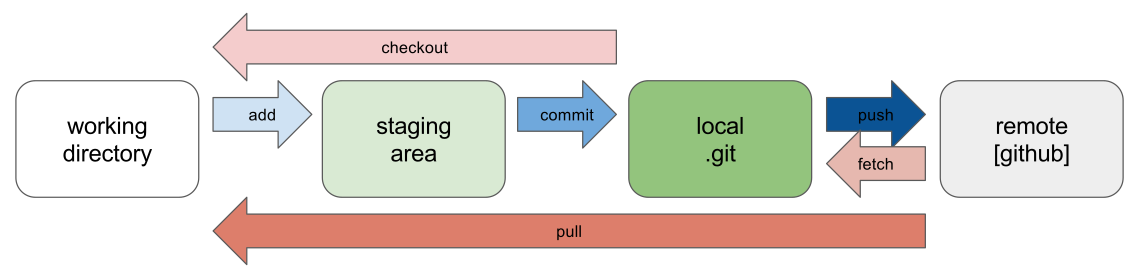
\includegraphics[scale=0.4]{pics/git-workflow}
    \caption{git workflow~\cite{git-workflow}}
    \label{fig:git-workflow}
\end{figure}

\cite{git-workflow}

\subsection{Semantische Versionierung}
\label{subsec:semantic-versioning}
Eine semantische Versionsnummer besteht aus drei Teilen:

\begin{center}
    \centering{MAJOR.MINOR.PATCH}
\end{center}

Und sollen nach Änderungen in der entsprechenden Kategorie in einser Schritten erhöht werden.

\textbf{MAJOR}
Wenn API Änderungen durchgeführt werden, welche die API mit der Vorgängerversion inkompatibel machen
\linebreak

\textbf{MINOR}
Wenn Funktionalität hinzugefügt wird, welche mit älteren Versionen noch kompatibel sind
\linebreak

\textbf{PATCH}
Wenn kleine Bug fixes durchgeführt werden, welche auch mit älteren Versionen kompatibel sind
\linebreak

Zusätzlich können auch labels für \emph{pre-release} oder \emph{build metadata} angegeben werden:

\begin{center}
    \centering{MAJOR.MINOR.PATCH format}
\end{center}

\cite{semantische-versionierung}

\subsection{GitHub}\label{subsec:github}
GitHub Inc. ist ein amerikanisches gewinnorientiertes Softwareunternehmen, welches git Repositories in der Cloud anbietet,
also das Remote Repository.
Dadurch können Privatpersonen aber auch große Unternehmen und Konzerne ganz leicht git als Versionierungstool verwenden.
Durch viele Features von GitHub wird das arbeiten mit git so stark erleichtert, dass auch Anfänger bereits sehr profesionell
mit git arbeiten und lernen können.
Normalerweise verwendet man git mit der Kommandozeile des jeweiligen Betriebssystemes, was hohes technisches Verständnis voraussetzt.
Man kann einen kostenlosen Account erstellen und gratis Repositories anlegen und verwenden,
deshalb ist Github in der Open-Source Community sehr stark verbreitet.
Doch mittlerweile kann diese Software mehr als "nur" Projekte zu versionieren.
Es gibt project-tracking-tools (GitHub Projects, Issues, Milestones, Labels, etc.), Pipelines für Continues Integration and Delivery,
gratis Website Hosting und noch vieles mehr~\cite{github-features}.

Es gibt aber auch andere Programme welche zu GitHub gehören, zum einen ist es \emph{Atom}, ein kostenloser und Open-Source Editor für Entwickler.
Weiters gibt es zum Beispiel auch \emph{Electron}, das ist ebenfalls ein Open-Source JavaScript Framework um Web-Anwendungen zu Desktopanwendungen zu machen.

Unternehmen können kostenpflichtige Organisationen anlegen, um alle Repositories einer Firma gesammelt an einem Ort zu verwalten.
Dazu gibt es wieder etliche Features welche die Sicherheit, Rollen und vieles mehr betreffen.

Seit 2018 gehört GitHub zu Microsoft, welche für die Übernahme \$7,5 Milliarden US-Dollar auf den Tisch gelegt haben~\cite{microsoft-acquires-github}.


\section{Projektkoordination}
\setauthor{Jonas Dorfinger}
Da Triply über eine GitHub Organisation verfügt, ist es naheliegend, dass für webmap ein eigenes Repository angelegt wird.

Um Übersicht über den Projektverlauf zu behalten, ist die Entscheidung aufgrund von internen Vereinbarungen von triply sowie die
Erfahrung des Teams auf GitHub Projects gefallen.
Man kann ein Project Board ganz einfach über die GitHub Website erstellen und dabei auswählen, ob eine Vorlage ausgewählt werden soll.

Es gibt folgende Templates zur Auswahl: ~\cite{github-create-project}

\paragraph{None}
Es wird ein völlig leeres Project Board erstellt, alle Spalten und Einstellungen müssen manuell gemacht werden.

\paragraph{Basic Kanban}
Ein Project Board mit den Spalten \emph{To do}, \emph{In progress} und \emph{Done} wird erstellt.

\paragraph{Automated Kanban}
Es wird ein Basic Kanban Board erstellt, mit der zusätzlichen Funktion von eingebauten Triggern, welche automatisch Issues
und Pull Requests zwischen den Spalten hin und her schieben.

\paragraph{Automated Kanban with Reviews}
Das Template \emph{Automated Kanban with Reviews} erweitert das Automated Kanban Template um 2 weitere Spalten und einen Trigger
, für die Pull Request Reviews.

\paragraph{Bug triage}
Dieses Template wird verwendet, um Bugs zu priorisieren und diese geordnet anzusehen, dabei gibt es folgende Spalten:

\begin{itemize}
    \item To do
    \item High priority
    \item Low priority
    \item Closed
\end{itemize}

\subsection{Issues}
Issues haben die Möglichkeit, die anstehende Arbeit zu dokumentieren und planen.

\cite{github-issues}

\subsection{Automatisierung}
Durch die Verwendung spezieller Keywords in Commit messages oder in einem Kommentar bei einem Issue, kann der Zustand dieses
Issues verändert werden.
Dies geht einher mit der Automatisierung von Project Boards.

\textbf{Keywords:}

\begin{itemize}
    \item close
    \item closes
    \item closed
    \item fix
    \item fixes
    \item fixed
    \item resolve
    \item resolves
    \item resolved
\end{itemize}

\textbf{Verwendung}

\begin{center}
    \centering{<Keyword> <Issue Nummer> <Commit Message>}
\end{center}

\cite{github-issue-automation}


\section{Frontend Framework/Library}
\label{sec:frontend-framework/library}
\setauthor{Jonas Dorfinger}
Webmap ist als Webanwendung konzeptioniert, deshalb ist es für das Frontend wichtig, eine Technologie zu wählen, welche
nicht nur langlebig ist, sondern auch eine gute Übersicht bietet.
Das beinhaltet unter anderem, dass eine große Community hinter dem Framework oder der Library steht,
aber auch die Anforderungen des Auftraggebers dürfen nicht unbeachtet bleiben.
Anhand dieser definierten Kriterien wurden die in 2021 beliebtesten Frameworks beziehungsweise Libraries verglichen.

\subsection{Framework vs. Library}
\label{subsec:framework-versus-library}
\setauthor{Jonas Dorfinger}
Sowohl Frameworks als auch Libraries sind Codes, welche oft auftretende Probleme einfach lösen sollen.
Um das konkret zu veranschaulichen, kann man dies mit einer Metapher besser beschreiben.

Eine Library ist wie der Besuch in einem Möbelhaus, man hat zwar grundsätzlich ein Haus aber keine Einrichtung, man
braucht also eine leichte Lösung um das Haus zu möblieren.
Einen Tisch selbst zu zimmern wäre zu aufwendig, deswegen wählt man einen Tisch aus der großen Auswahl in dem besuchten Geschäft.

Das Verwenden eines Frameworks ist wie der Bau eines Hauses, man hat ein paar Blaupausen und Vorgaben zum Design und zur
Architektur des neuen Gebäudes.
Es wird also ein Grundgerüst zur Verfügung gestellt, in welchem man den Regeln konform frei agieren kann.

Zusammengefasst sind Frameworks Gerüste, welche durch Entwickler projektspezifisch erweitert werden müssen und Libraries
fertige Pakete, mit denen Programmierer Anwendungen um spezielle Funktionen erweitern.

\subsection{Angular}
\label{subsec:angular}
\setauthor{Jonas Dorfinger}
Angular wurde 2016 von Google ins Leben gerufen, seitdem ist es ein beliebtes Framework für die Webentwicklung.
Nur auf TypeScript basierend füllt es die Lücke zwischen der wachsenden Nachfrage von Technologien und traditionellen
Ideen zur Performance Optimierung.
Die Entwicklerplattform bietet etliche Services und Features an, dazu gehören nicht nur der Cross-Platform Support,
sondern auch eine built-in Geschwindigkeits- und Performanceoptimierung.
Auch für Unternehmen mit sehr hohen Nutzerzahlen ist Angular ein gern gewähltes Tool.
Ein großer Vorteil von Angular ist zudem, dass es unter einer Open-Source-Lizenz veröffentlicht
ist und somit nicht von dem Angular-Google Team, sondern auch von der Community betreut und erweitert wird.
Angular hat mit dem Two-Way-Binding einen großen Vorteil gegenüber React~\ref{subsec:react}.
Dieses Feature stellt sicher, dass die View und das Model in Echtzeit miteinander synchronisiert werden.
Das bedeutet, dass eine Änderung im Model direkt in der View angezeigt wird, aber auch eine Änderung in der View direkt
ins Model übertragen wird.
~\cite{angular-features,what-is-angular}

\paragraph{Vorteile}
\begin{itemize}
    \item Features und Funktionalität wie das Two-Way-Binding sind direkt inkludiert
    \item Direkt eingebaute Features zum Updaten der View oder des Models
    \item Komfortable Wiederverwendung von Components durch Dependency Injection
    \item Große Community zum Lernen und zur Fehlersuche
\end{itemize}

\paragraph{Nachteile}
\begin{itemize}
    \item Schwieriger zu lernen, da Angular sehr umfangreich ist und es viele mögliche Lösungen gibt
    \item Durch die riesigen und komplexen Strukturen kann es sein, dass bei großen dynamischen Applikationen Performance Probleme auftreten
    \item Angular ist ein full-package Framework, weshalb es für kleine Applikationen ungeeignet ist
\end{itemize}

\subsection{React}
\label{subsec:react}
\setauthor{Jonas Dorfinger}
ReactJS ist die größte Konkurrenz von Angular, mit einem Vielfachen an Marktanteilen.
Im Gegensatz zu Angular wird React von Facebook gewartet und betreut und verfügt über die Funktionalität des virtuellen
Document Object Models (DOM).
Das virtuelle DOM verbessert die Performance und verringert die Dauer von Render Prozessen, da nur die Inhalte verwendet werden,
welche sich auch tatsächlich verändert haben und nicht die gesamte View neu gerendert wird.
Durch dieses Feature wird eine Plattform geschaffen, welche sich sehr gut für Applikationen mit großem Traffic eignet.
Ein Alleinstellungsmerkmal ist dazu auch noch, dass React Server-Side Rendering unterstützt.
Für SPAs, also Single Page Applications ist es empfehlenswert sich für React zu entscheiden, durch das Wiederverwenden der
Komponenten kann man in kurzer Zeit gute und interaktive User Interfaces entwickeln.

\begin{figure}[hbt!]
    \centering
    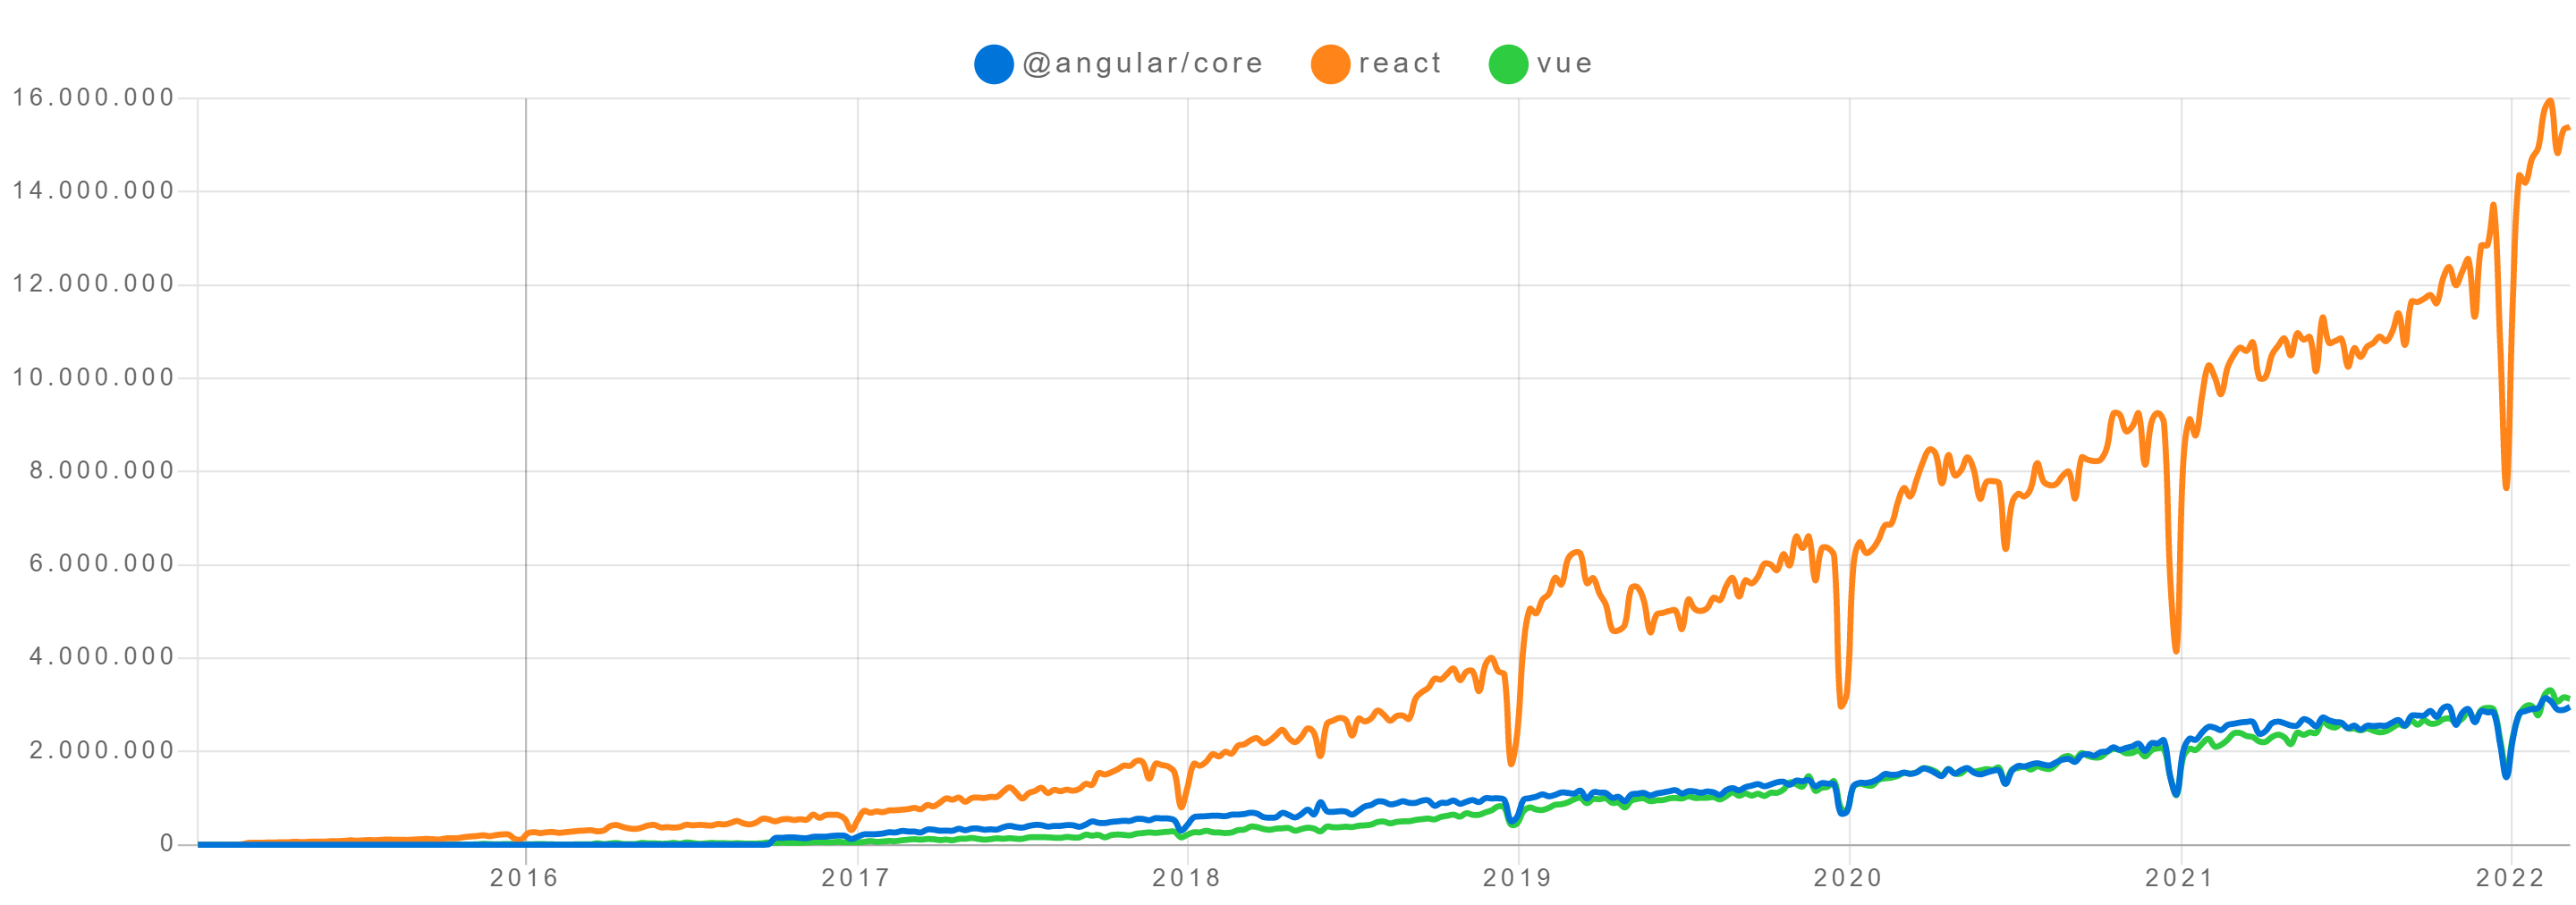
\includegraphics[scale=0.15]{pics/angular-react-vue-npm-chart}
    \caption{wöchentliche Downloads~\cite{angular-react-vue-stats}}
    \label{fig:angular-react-vue-chart}
\end{figure}
\begin{figure}[hbt!]
    \centering
    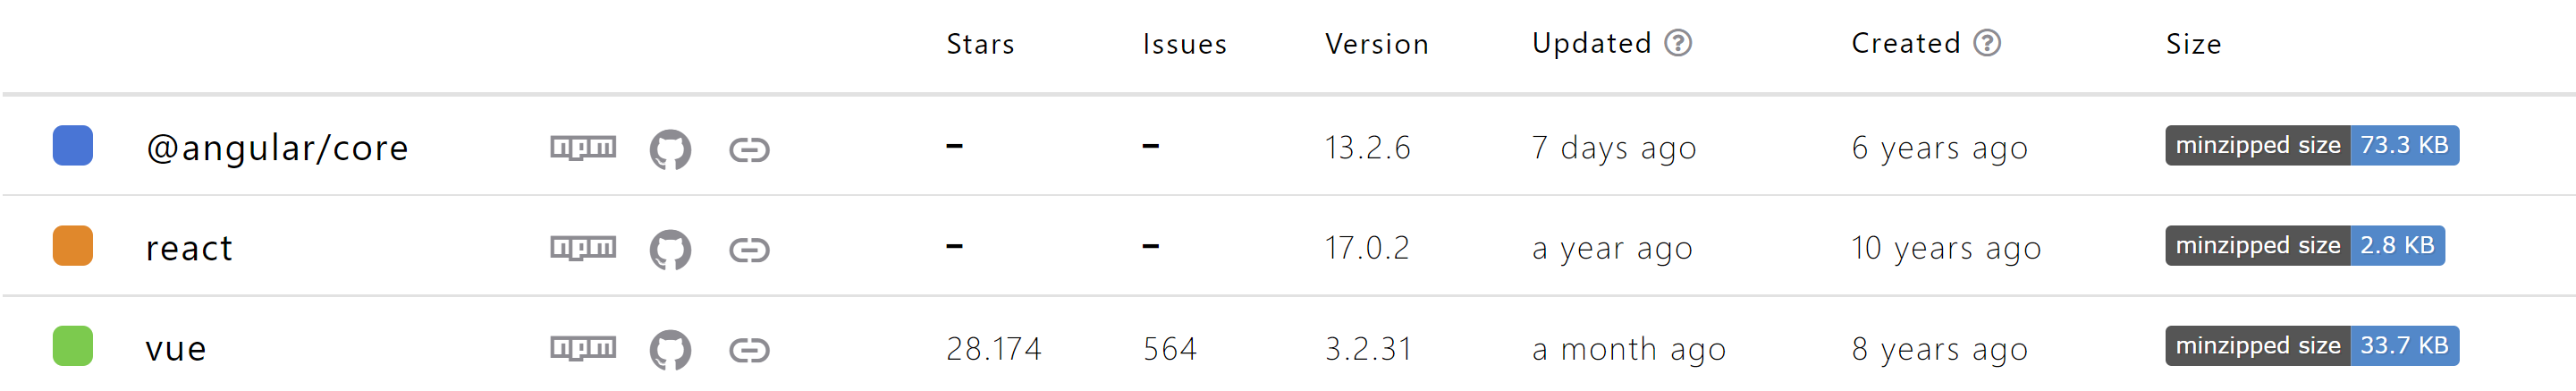
\includegraphics[scale=0.5]{pics/angular-react-vue-npm-stats}
    \caption{Direkter Vergleich der Frameworks~\cite{angular-react-vue-stats}}
    \label{fig:angular-react-vue-stats}
\end{figure}

\paragraph{Vorteile}
\begin{itemize}
    \item Durch das virtuelle DOM ist die Performance sehr optimiert und kann gut mit vielen gleichzeitigen Zugriffen zurechtkommen
    \item Unabhängige Components sind leicht zu implementieren und wiederzuverwenden
    \item React Developer Tools sind mit einer großen Nutzbarkeit sehr ausgereift
\end{itemize}

\paragraph{Nachteile}
\begin{itemize}
    \item Durch etliche Updates ist die Dokumentation lückenhaft
    \item Schnelle Änderungen in kurzer Zeit, neu gelerntes ist in naher Zukunft bereits wieder "alt"
    \item Inhalte wie JSX sind komplex und schwer zu lernen
    \item ReactJS setzt einiges an Erfahrung in JavaScript oder TypeScript voraus
\end{itemize}

\subsection{Vue}
\label{subsec:vue}
\setauthor{Jonas Dorfinger}
Vue.js ist ein kleines, aber sehr einfach funktionierendes Frontend System und wird immer beliebter.
Es ist gut sehr darin, Probleme mit denen Angular Developer umgehen müssen zu vermindern oder gar zu lösen.
Vue.JS ist außerdem sehr leichtgewichtig und klein, hat aber trotzdem viele nützliche Features wie das Two-Way-Binding
out-of-the-box dabei, auch die Verwendung als PWA (Progressive Web Apps) ist möglich.
Der wohl größte Nachteil ist die niedrige Trucknumber~\cite{truck-factor-of-popular-github-projects, what-is-the-bus-factor}.
Bei Projekten beschreibt dies, wie viele Personen ausfallen können, damit das Projekt weiterlaufen kann.
Je höher die Trucknumber, desto mehr Personen könnten ausfallen und das Projekt würde trotzdem weiterlaufen.
Im Gegensatz dazu, je kleiner die Trucknumber, desto weniger Personen können ausfallen.
Das geht so weit, dass das gesamte Projekt an einer einzigen Person hängt.
Das letzte Beispiel ist fast bei Vue.js gegeben, in das Core Repository von Vue committed regelmäßig nur der Gründer
von Vue, Evan You.
VueJS kann in beiden, TypeScript und JavaScript geschrieben werden.

\paragraph{Vorteile}
\begin{itemize}
    \item Sehr leicht zu lernen, vor allem mit basis JavaScript Wissen
    \item Flexibles App Layout
    \item Umfangreiche und ausführliche Dokumentation
\end{itemize}

\paragraph{Nachteile}
\begin{itemize}
    \item Sehr kleine Community (Wartung und Support)
    \item Sehr geringe Truck Number
    \item Stabilitätsprobleme bei großen Projekten
\end{itemize}

\begin{figure}[hbt!]
    \centering
    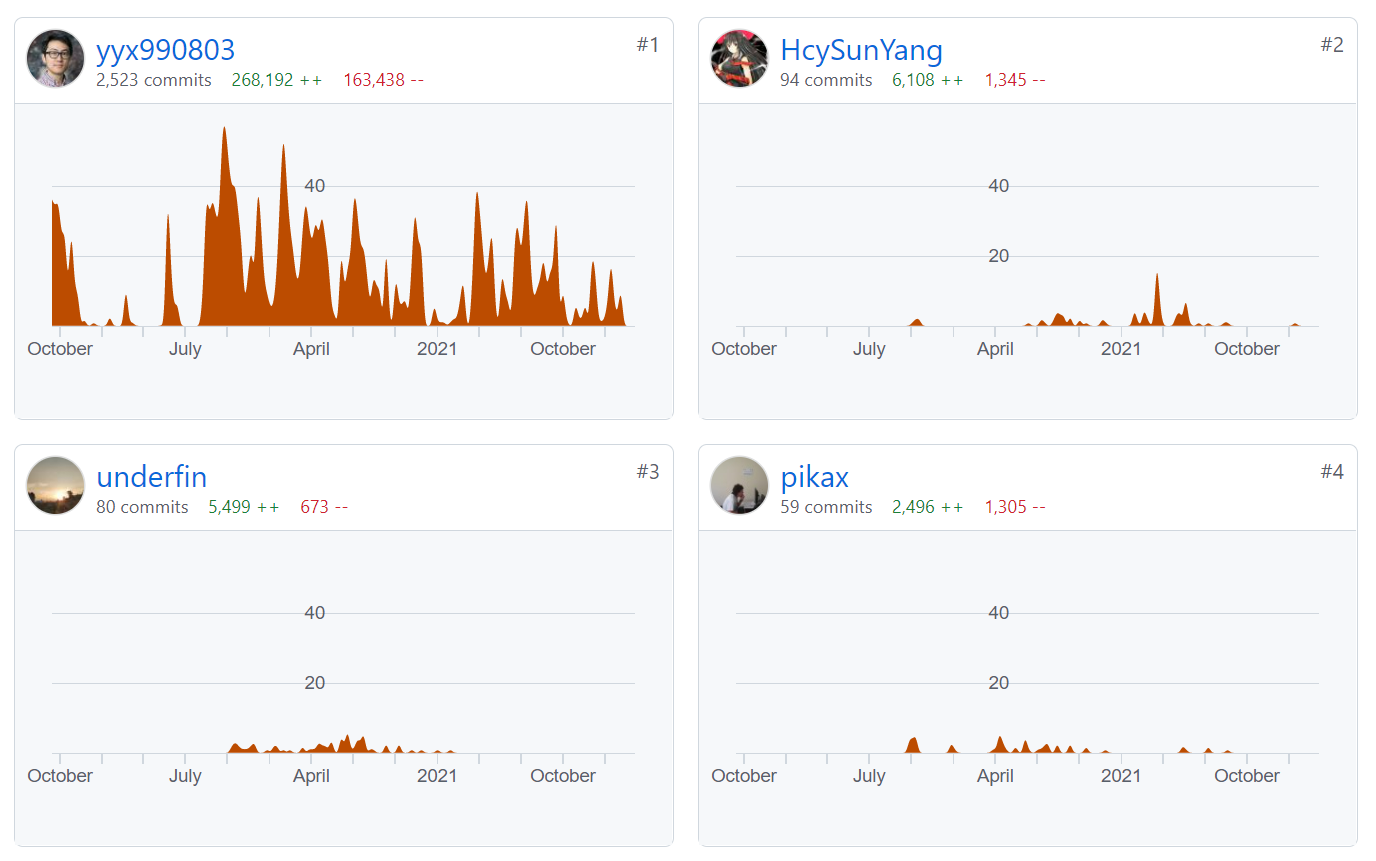
\includegraphics[scale=0.8]{pics/vue_contributions}
    \caption{Vue.js Core Repository Commits im Zeitraum 16. September 2018 - 9. Februar 2022~\cite{VueJSContribution}}
    \label{fig:vue_contributions}
\end{figure}

~\cite{best-frontend-frameworks, best-frontend-framework-2022, angular-vs-react-vs-vue}

\subsection{Verwendung von Angular}
\setauthor{Jonas Dorfinger}

\subsubsection{Warum Angular?}
\setauthor{Jonas Dorfinger}
Einer der Entwickler hat bereits mehr als zweieinhalb Jahre Erfahrung in der Entwicklung von UserInterfaces und Web-Oberflächen mit Angular.
Zusätzlich dazu wird Angular in der HTL Leonding ab dem 4. Jahrgang in der Abteilung Medientechnik unterrichtet, wodurch
die Wahl auf dieses Framework naheliegend war.
Unabhängig von der Schule und den Entwicklern ist es außerdem eine Anforderung der Betreuerfirma triply Angular zu verwenden.
Triply vertraute bisher bei allen Frontend Projekten auf Angular.

\subsubsection{Angular installieren und verwenden}
\setauthor{Jonas Dorfinger}

\paragraph{Node.js}
\label{Node.js}
Node.js ist eine asynchrone open-source Event gesteuerte JavaScript Entwicklerumgebung.
Node.js ist Plattformunabhängig, das heißt, dass in node geschriebene Anwendungen sowohl auf Windows oder Linux als auch auf macOS problemlos funktionieren.
JavaScript wird grundsätzlich im Browser ausgeführt, durch node kann JavaScript jedoch auch serverseitig ausgeführt werden.
Dabei erhält man durch die Node.js API umfangreiche Funktionen, um mit dem lokalen Betriebssystem zu interagieren.
Node.js wird verwendet, um skalierbare Netzwerk Applikationen zu designen.
Im folgenden Beispiel wird gezeigt, wie man einen einfachen Node.js Webserver implementiert.
Durch diese Implementierung können etliche Verbindungen gleichzeitig behandelt werden.
Bei jeder Verbindung wird die Callback Funktion ausgeführt.
Werden keine Verbindungen aufgebaut, so geht Node.js in den Wartezustand.
Wenn man Node.js verwendet, muss man sich keine Sorgen über dead-locks machen, weil es durch die Asynchronität keine locks gibt.
Node.js Funktionen führen kaum I/O Prozesse durch,
dadurch kann ein Prozess nie blockieren außer es wird die I/O Funktion synchron über die Node.js Library aufgerufen.
Weil keine Prozesse blockieren, ist es naheliegend skalierende Systeme in Node.js zu entwickeln~\cite{about-node-js}.

\begin{lstlisting}[label={lst:hello-world.js}]{hello-world.js}
const http = require('http');

const hostname = '127.0.0.1';
const port = 3000;

const server = http.createServer((req, res) => {
  res.statusCode = 200;
  res.setHeader('Content-Type', 'text/plain');
  res.end('Hello World');
});

server.listen(port, hostname, () => {
  console.log(`Server running at http://${hostname}:${port}/`);
});
\end{lstlisting}

\paragraph{npm}
npm oder auch ausgeschrieben der Node-Package-Manager ist eine Software um Packages zu Node.js Applikationen hinzuzufügen.
npm wird standardmäßig mit Node.js mitinstalliert, es handelt sich um eine CLI (Command-Line-Interface) welche auf die online registry zugreift.
Die npm-registry ist eine Online-Datenbank welche public (open-source) und private (auch kostenpflichtige) Packages zur Verfügung stellt.
Die Packages werden über die CLI installiert und können über die \href{https://npmjs.com}{npm Website} gesucht werden.
npm ist ein Produkt von Github, Github wiederum gehört seit 2018 zu Microsoft~\cite{microsoft-acquires-github}.

\paragraph{TypeScript}
\label{TypeScript}
TypeScript ist eine typisierte Programmiersprache welche auf JavaScript aufbaut.
TypeScript ist außerdem eine Übermenge von JavaScript.
Das bedeutet, dass TypeScript alle Eigenschaften von JavaScript hat und zusätzlich noch eigene Funktionalität mitbringt.
Folgende Features werden im Gegensatz zu JavaScript unterstützt:

\begin{itemize}
    \item Typisierung von Variablen (auch während des Kompilierens)
    \item Type inference
    \item Type erasure
    \item Interfaces
    \item Enumerated types
    \item Generics
    \item Namespaces
    \item Tuples
    \item Async/await
    \item Classes
    \item Modules
    \item Verkürzte Syntax von anonymen arrow-functions
    \item Optionale Parameter and Defaultwerte für Parameter
\end{itemize}

Wenn man ein TypeScript Programm ausführt, dann wird der Quellcode von TypeScript Code in JavaScript Code transpiled.
Dies wird erzielt, indem eine von mehreren möglichen Optionen ausgewählt wird.
Die Auswahl beschränkt sich dennoch auf den TypeScript Checker oder Babel, beide Varianten sind stark verbreitet.
TypeScript kann sowohl clientseitig, als auch serverseitig (zum Beispiel in Kombination mit Node.js) eingesetzt werden.

\paragraph{Beispiel: Funktionen mit und ohne Types} \

JavaScript Funktion zum Addieren von 2 Zahlen (ohne types)
\begin{lstlisting}[label={lst:add-function-js}]{app.js}
function add(number1, number2) {
    return number1 + number2;
}


add(6, 9);  // returns 15

add("Hallo ", "Welt");  // returns "Hallo Welt"
\end{lstlisting}

Bei JavaScript gibts es keine typisierten Funktionen, deshalb verhält sich die Funktion immer den Parametern entsprechend.

\

TypeScript Funktion zum Addieren von 2 Zahlen (mit types)
\begin{lstlisting}[label={lst:add-function-ts}]{app.ts}
function add(number1: number, number2: number): number {
    return number1 + number2;
}

add(6, 9);  // returns 15

add("Hallo ", "Welt");  // Error: Argument of type 'string' is not assignable to parameter of type 'number'.
\end{lstlisting}

Da TypeScript Typisierungen unterstützt, wird bereits zur Compilezeit sichergestellt, dass die richtigen Daten als Parameter übergeben werden.
Deshalb tritt beim zweiten Aufruf ein Error auf, weil ein String nicht als Nummer verwendbar ist.

\cite{typescript-landing-page, what-is-typescript}

\subsubsection{Wie funktioniert Angular?}
\setauthor{Jonas Dorfinger}
\emph{Ivy} ist die neue Compilation und Rendering Pipeline für Angular.
Seit der Angular Version 9 wird standardmäßig die neue Pipeline verwendet und ersetzt damit die Alter Pipeline,
welche unter dem Namen \emph{View Engine} bekannt ist.

Da \emph{Ivy} nicht nur eine Rendering Engine, sondern auch eine Compile Engine ist, öffnen sich ganz neue Türen was die
Optimierung für und über das gesamte Framework angeht.

Anstatt Template Daten zu generieren, diese in einen Interpreter zu geben, der wiederrum entscheidet, welche Operationen
ausgeführt werden, wird direkt eine Sammlung an \emph{Template Instructions} generiert.
Die \emph{Template Instructions} beinhalten die Logik, welche Components instanziiert, DOM Nodes erstellt und Change Detection in Echtzeit ausführt.

\begin{figure}[hbt!]
    \centering
    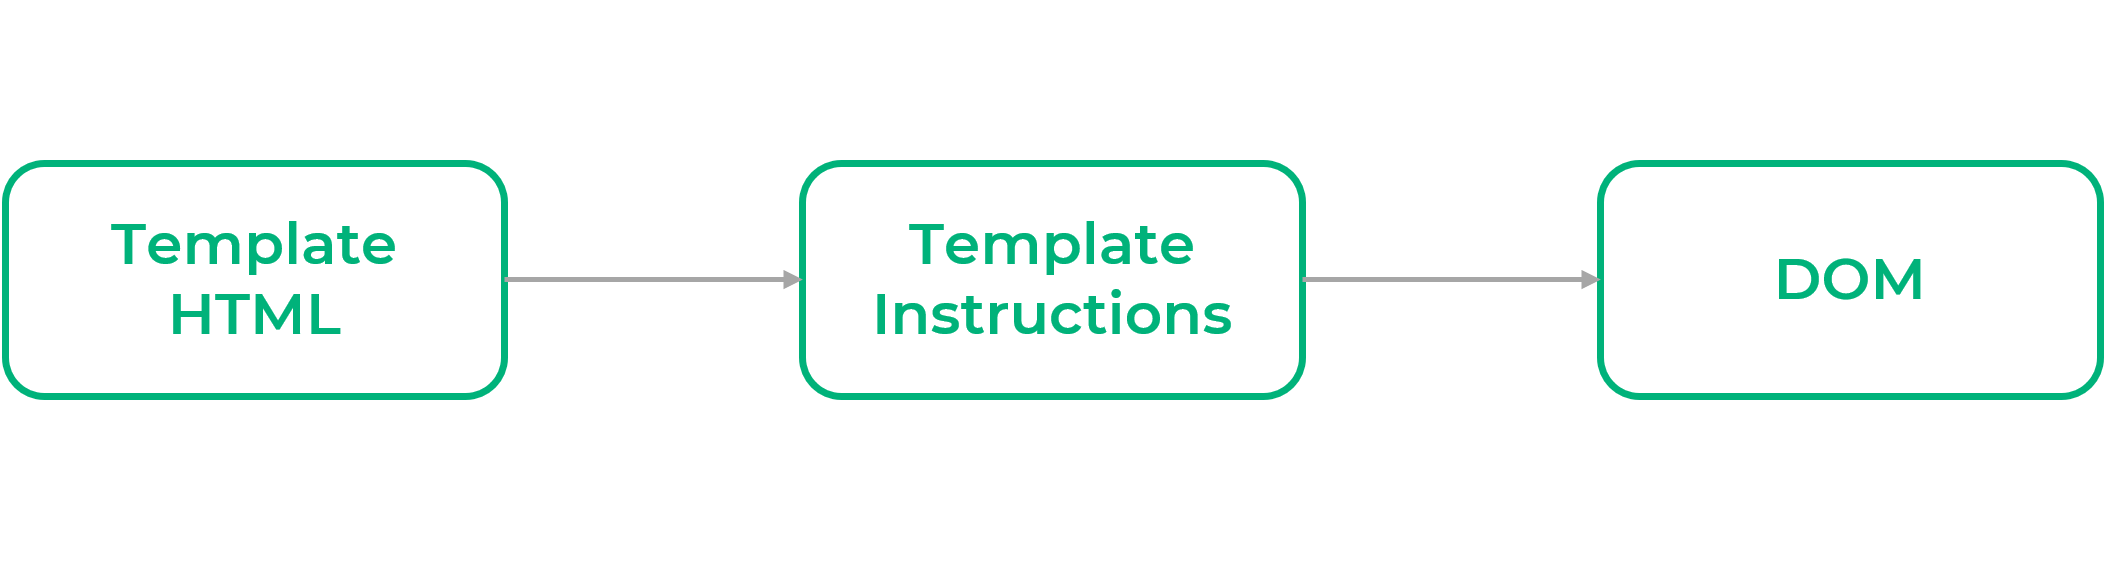
\includegraphics[scale=.4]{pics/ivy-pipeline}
    \caption{Ivy Pipeline}
    \label{fig:ivy-pipeline}
\end{figure}

\paragraph{Incremental DOM}
Jede Component wird in eine eigene Sammlung an Instructions compiled, diese erstellen DOM Trees und aktualisieren die
Daten an Ort und Stelle, wenn diese sich ändern.
Zum Erstellen des \emph{Document Object Models} gibt es drei verschieden Funktionen:

\begin{itemize}
    \item \emph{elementStart} (opening tag)
    \item \emph{text} (inner html)
    \item \emph{elementEnd} (closing tag)
\end{itemize}

Beim Aktualisieren des DOMs wird nicht automatisch jedes Mal ein komplett neuer Tree erstellt, sondern es werden alle
Nodes verglichen und nur jene verändert, welche auch tatsächlich verändert wurden.
Das spart nicht nur Arbeitsspeicher, sondern auch Zeit.

Der Grund warum Incremental DOM verwendet sind die Ziele welche erreicht werden möchten.
Der Fokus liegt auf einer besseren Performance von Web-Applikationen auf Mobilen Endgeräten (Handys, Tablets).
Um dies zu erreichen, ist es erforderlich zwei Dinge zu optimieren, \emph{bundle size} und \emph{memory footprint}.


\paragraph{Shakable Tree}
Bei Verwendung der Incremental DOM Strategie wird nicht die Component interpretiert, sondern jede Component verweist auf
verschiedene Instructions.
Wenn kein Verweis auf eine Instruction zu finden ist, dann wird dieser Teil nicht verwendet und ist somit überflüssig.
Durch die Vorteile von Incremental DOM ist dies bereits zur Compile Zeit bekannt, weshalb alle nicht benützten Instructions
vom bundle entfernt, was wiederrum die \emph{bundle size} beträchtlich verringern kann.

\begin{figure}[hbt!]
    \centering
    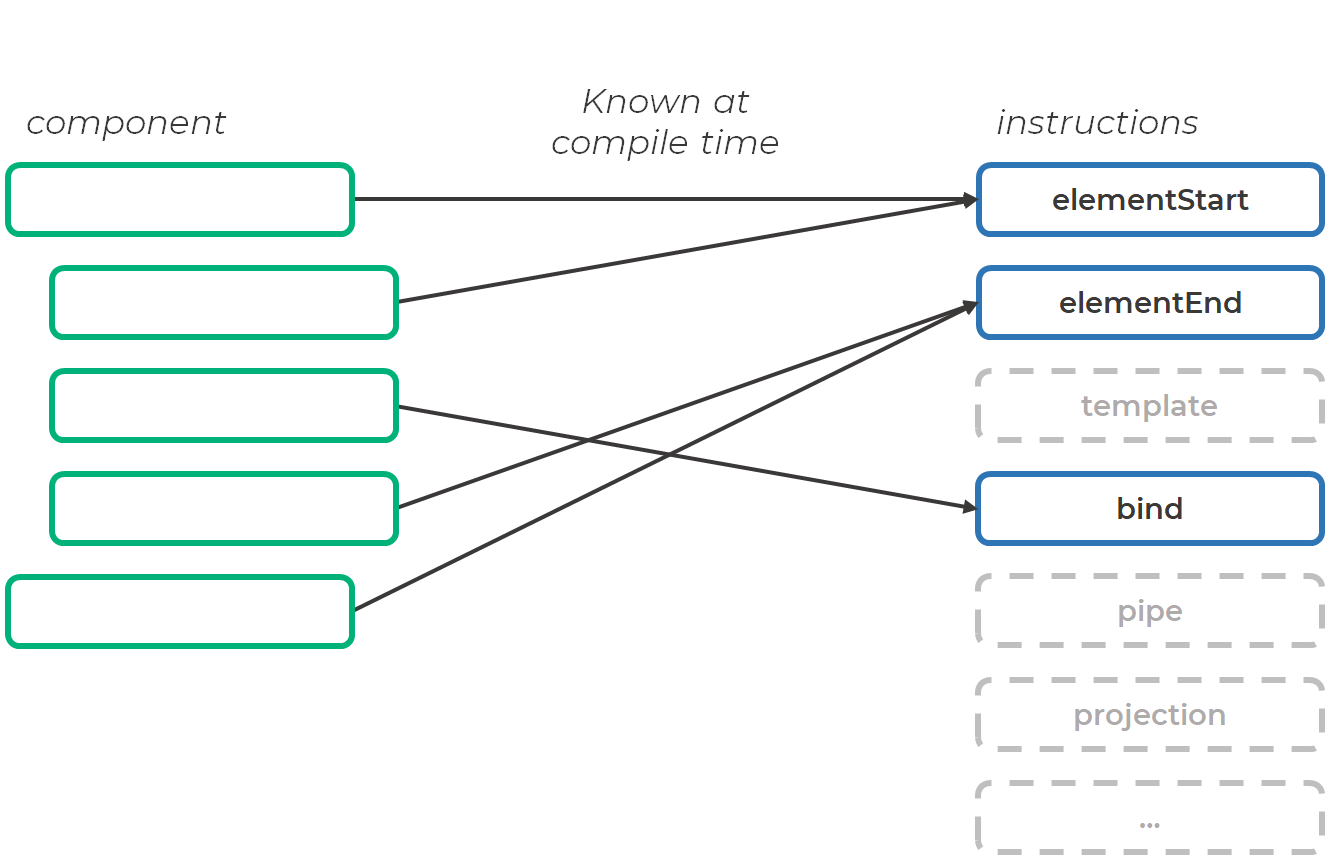
\includegraphics[scale=.6]{pics/shakable-tree}
    \caption{Skakable Tree}
    \label{fig:shakable-tree}
\end{figure}

\cite{rendering-engine-ivy, incremental-dom}

\cleardoublepage

\subsubsection{Angular Material}
\setauthor{Jonas Dorfinger}
Angular Material ist eine Component-Library von Angular, diese beinhaltet stylistisch aufeinander abgestimmte Elemente.
Diese Komponenten können ganz einfach importiert werden. Durch das Responsive Design der Inhalte, eignen sich diese sehr gut
für die Umsetzung einer Web-Oberfläche, da nicht viel Zeit für das Design verloren geht, sondern der Fokus voll und ganz
auf die Funktionalität gelegt werden kann.

Angular Material kann jederzeit über einen Konsolenbefehl zu einem Angular Projekt hinzugefügt werden:
\begin{center}
    \centering{ng add @angular/material}
\end{center}

Bei der Installation kann man bereits vordefinierte Themes von Angular auswählen, zur Auswahl stehen insgesamt 4 verschiedene,
zwei Dark- und zwei Lighttheme Varianten~\cite{angular-material-predefined-themes}:

\begin{itemize}
    \item Deep Purple \& Amber (Light)
    \item Indigo \& Pink (Light)
    \item Pink \& Blue-grey (Dark)
    \item Purple \& Green (Dark)
\end{itemize}

Weiters hat man die Möglichkeit eigene Themes zu erstellen.
Mithilfe von Custom Themes können die von Angular bereitgestellten Komponenten für jedes Projekt individuell eingefärbt werden.
Um das zu erreichen, wählt man beim Installieren die fünfte Auswahlmöglichkeit \emph{Custom} aus.
Dies erstellt den dafür benötigten Code in dem \emph{styles.scss} File.
Man kann sich über diverse Internet Seiten Farbpaletten generieren lassen, diese werden benötigt, um ein eigenes Theme zu gestalten.
Ein Angular Theme hat genau "drei" verschieden Farben, wobei es eher Farbpaletten sind.

\paragraph{primary-palette}
Die Primary Palette legt die Hauptfarbe fest, welche in fast allen Komponenten standardmäßig verwendet wird.
Man kann allerdings auch bei den meisten Komponenten individuell als Parameter angeben, welche der drei Paletten verwendet werden soll.

\paragraph{accent-palette}
Die Accent Palette definiert eine Akzentfarbe, welche einen hohen Kontrast zur Hauptfarbe haben soll, um bestimmte Elemente
besser hervorheben zu können.

\paragraph{warn-palette}
Die Warn Palette besteht meist aus einem Rot, welcher für Fehlermeldungen verwendet wird.

\linebreak
\linebreak
\linebreak

Eine Farbpalette besteht aus einer Basisfarbe und mehreren Abstufungen dieser Farbe, um auch hier unterschiedliche Töne für
Hervorhebungen zu haben.

Ein Beispiel einer Farbpalette für eine primary-palette:

\begin{lstlisting}[label={lst:custom-primary-color-palette}]{style.scss}
$primary-palette: (
  50 : #e2f3f4,
  100 : #b8e2e4,
  200 : #88ced2,
  300 : #58babf,
  400 : #35acb2,
  500 : #119da4,
  600 : #0f959c,
  700 : #0c8b92,
  800 : #0a8189,
  900 : #056f78,
  A100 : #a7f7ff,
  A200 : #74f3ff,
  A400 : #41efff,
  A700 : #27ecff,
  contrast: (
    50 : #000000,
    100 : #000000,
    200 : #000000,
    300 : #000000,
    400 : #000000,
    500 : #ffffff,
    600 : #ffffff,
    700 : #ffffff,
    800 : #ffffff,
    900 : #ffffff,
    A100 : #000000,
    A200 : #000000,
    A400 : #000000,
    A700 : #000000,
  )
);
\end{lstlisting}

Insgesamt hat man die Auswahl aus 36 verschiedenen Komponenten~\cite{angular-material-component-overview,angular-material-description,angular-material-with-angular}.

Die Komponenten werden ganz einfach über einen Custom HTML Tag eingebunden.

\subsubsection{triply Material Library}
\setauthor{Jonas Dorfinger}
Triply hat in den letzten Monaten einige eigene Angular Komponenten erstellt und in einer internen Bibliothek gesammelt.
Auf diese Inhalte wurde besonders zurückgegriffen, um zum Beispiel einen Slider oder einen true/false Switch
zu verwenden.
Der Unterschied zu Angular Material liegt darin, dass die Firmeninterne Library aus Files besteht, welche in das Projekt
kopiert werden, vereinfach gesagt, dass dabei Custom-Components verwendet werden.

\begin{figure}[hbt!]
    \centering
    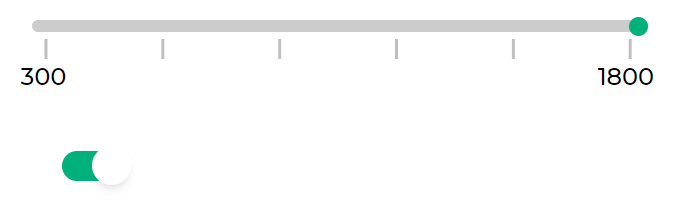
\includegraphics[scale=1]{pics/triply-material-library}
    \caption{Triply Slider und Triply Switch}
    \label{fig:triply-material-library}
\end{figure}

\subsubsection{Model-View-Controller Design Pattern}
\setauthor{Jonas Dorfinger}
Dieses Pattern wird oft für die Entwicklung von User Interfaces verwendet,
dabei wird die Logik in drei verschiedenen Elementen (Files) aufgeteilt.
Das hat zum Ziel, interne Abbildungen und Referenzen von Daten beziehungsweise Informationen
in einer Art und Weise aufzuteilen.
Das Model ist von der restlichen Anwendung komplett
unabhängig.
Im Gegensatz dazu ist die View stark abhängig von der zu programmierenden Anwendung.
Die Aufgabe der View beschränkt sich rein auf die Visualisierung der durch den Controller bereitgestellten Daten.
Der Controller hat eine Vermittlerrolle zwischen Model und View.
In Angular ergeben alle drei Files eine gemeinsame Component.

\paragraph{Model}
Das Model File ist das Herzstück der Component, es beinhaltet alle Daten
Strukturen und den Aufbau, dabei werden Daten, Logik und Regeln
der Component festgelegt und verwaltet.
Bei Angular sind das entweder Interfaces oder Klassen ohne Logik.
~\cite{angular-design-patterns}

\paragraph{View}
Die View beinhaltet alle Details zur Darstellung der Daten und Informationen.
Es kann mehrere Views für die gleiche Information geben, zum Beispiel ein
Balkendiagramm für den Manager oder eine Tabelle für die Buchhaltung.

\paragraph{Controller}
Der Controller ist das Gehirn einer Component, er ist das Verbindungsstück zwischen View und Model.
Dabei werden die Daten mittels Getter-Funktionen aus dem Model geladen und so verändert beziehungsweise manipuliert, dass die View diese richtig
anzeigen kann.
Wenn dadurch Änderungen der Daten gemacht werden, speichert der Controller diese Änderung mittels Setter-Funktionen im Model.

\begin{figure}[hbt!]
    \centering
    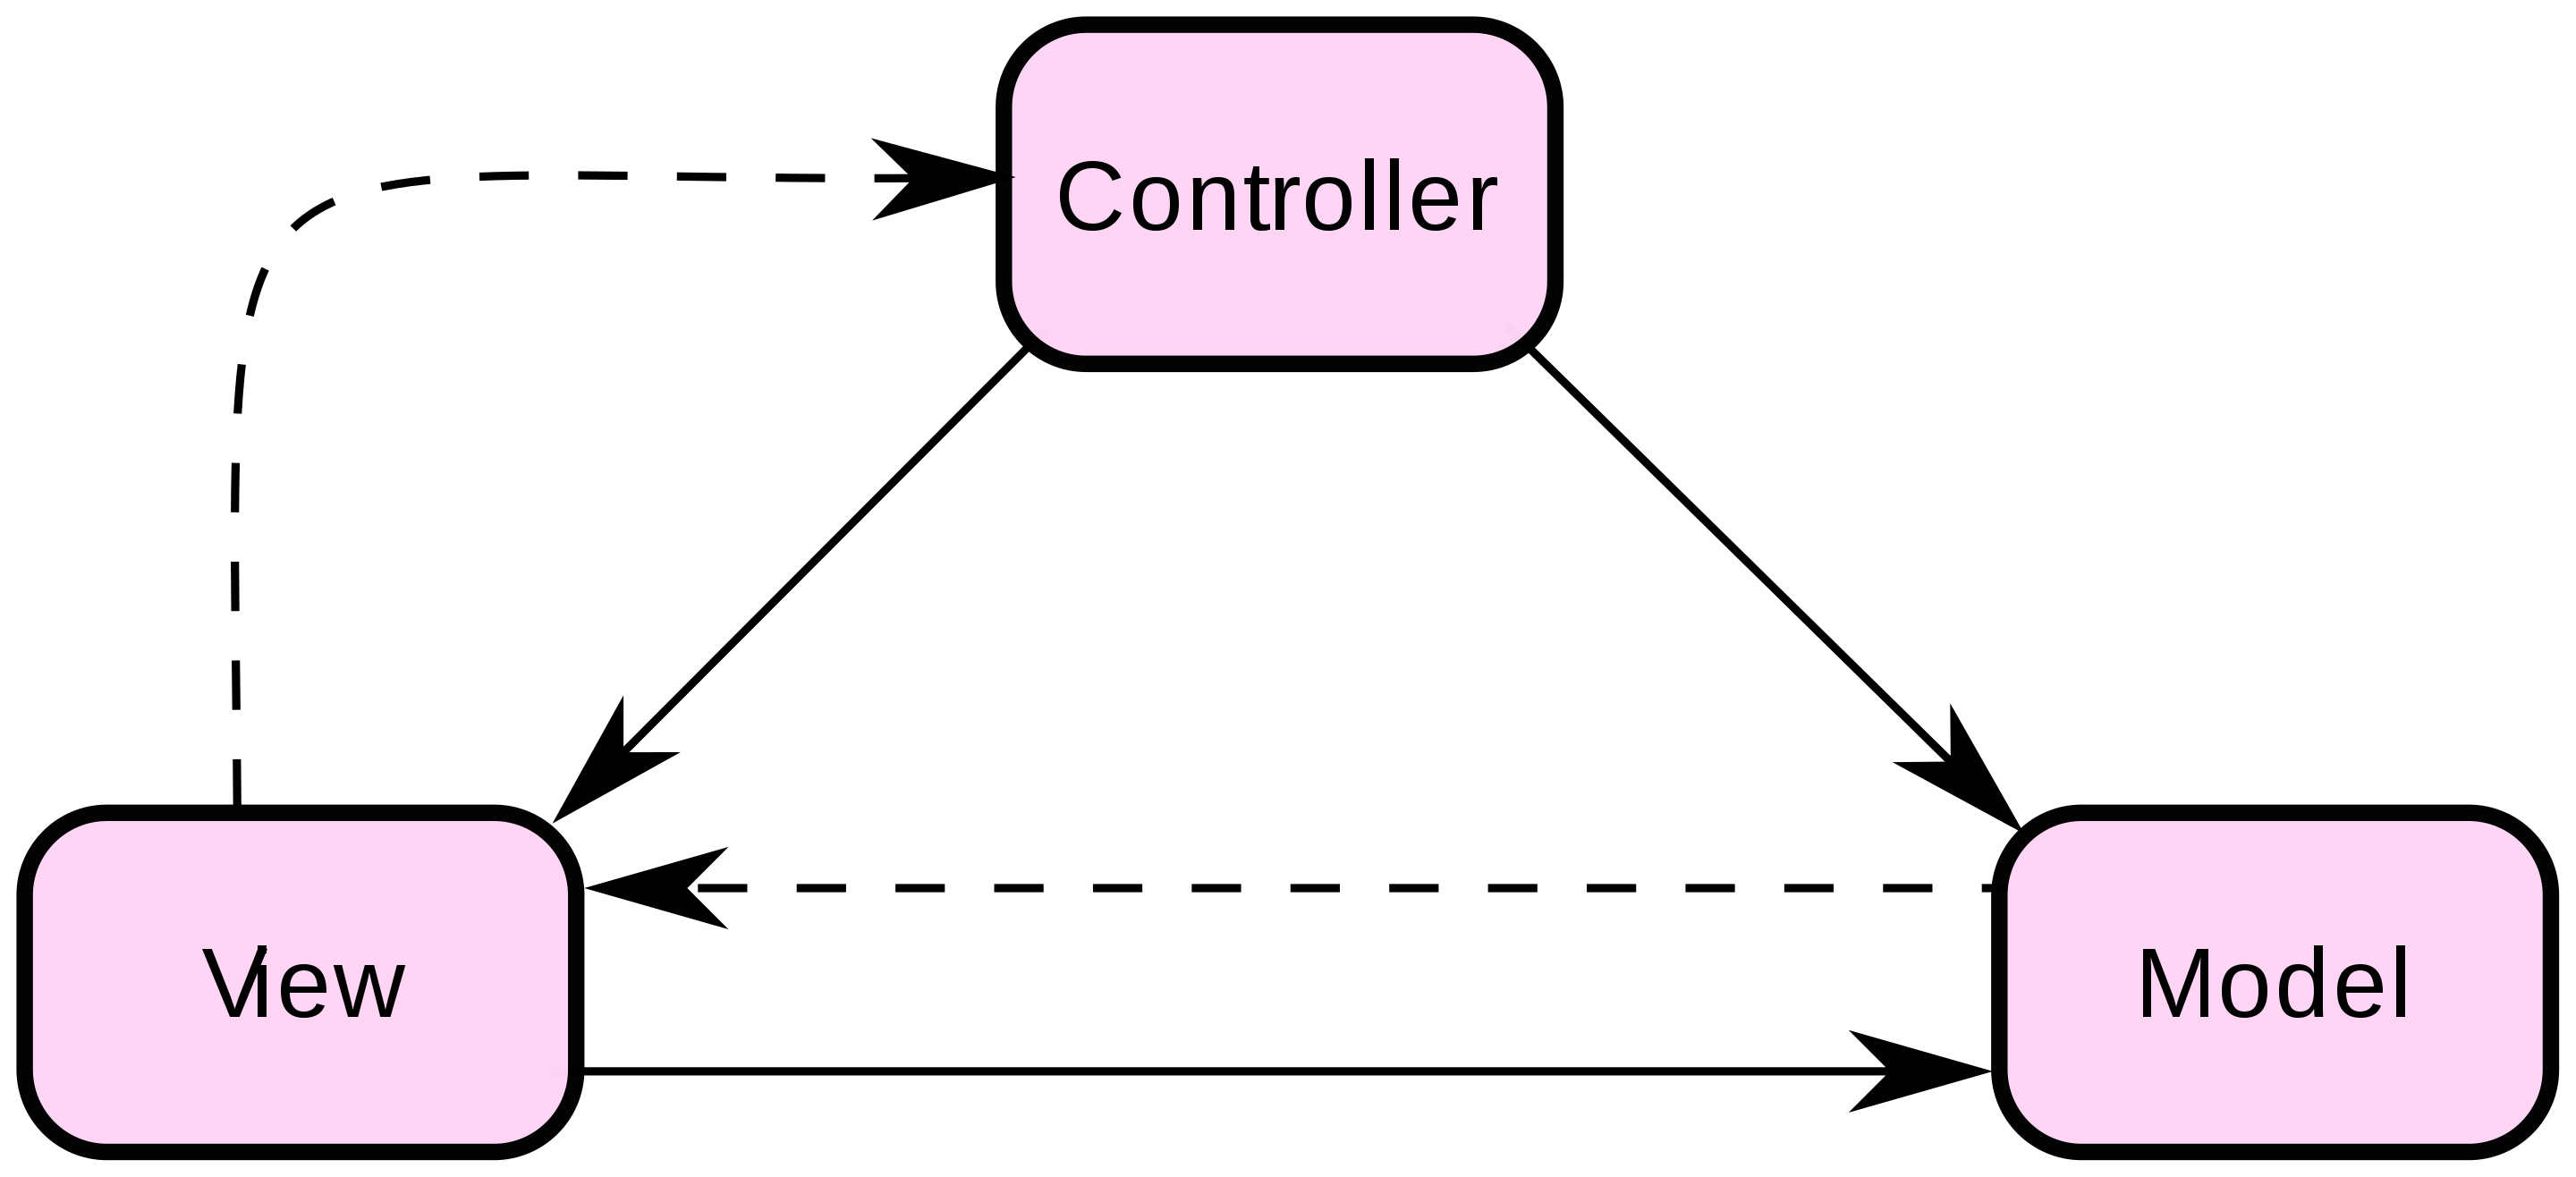
\includegraphics[scale=0.1]{pics/mvc_design_pattern}
    \caption{Model-View-Controller-Pattern}
    \label{fig:mvc_design_pattern}
\end{figure}



\section{Map Frameworks}
\setauthor{Jonas Dorfinger}
Geo-Daten sind sehr komplexe Daten, welche nur sehr schwer und mit viel Erfahrung ohne Visualisierung interpretiert werden können.
Um solche Daten visualiseren zu können werden Map Frameworks benötigt, diese können auf digitalen Karten, die Koordinaten
grafisch darstellen, doch auch interaktive Darstellungen sind möglich.
Drei der bekanntesten Frameworks sind:

\begin{itemize}
    \item Mapbox
    \item Leaflet
    \item Google Maps
\end{itemize}

\subsection{Mapbox}
Mapbox ist ein amerikanisches Unternehmen, welches sich auf Custom-Maps spezialisiert und die Nische stark vergrößert hat.
Dabei geht es um die Darstellung von Geo-Daten auf digitalen Kartensystemen und deren Individualisierung.
Weiters ist Mapbox Contributor zum OpenStreetMap (OSM) Projekt, das ist eine Geo-Datenbank mit Kartendaten und Informationen
für den gesamten Globus.
Große Konzerne wie Amazon, Facebook oder Snapchat setzen auf OpenStreetMap für ihre eigenen Angebote und Services den Kunden gegenüber.
Unternehmen wie Tesla, mit einer eigenen Navigationssoftware verwenden die OSM-Datenbank ebenfalls für ihre eigenen Zwecke~\cite{osm-customers-1, osm-customers-2}.

\begin{figure}[hbt!]
    \centering
    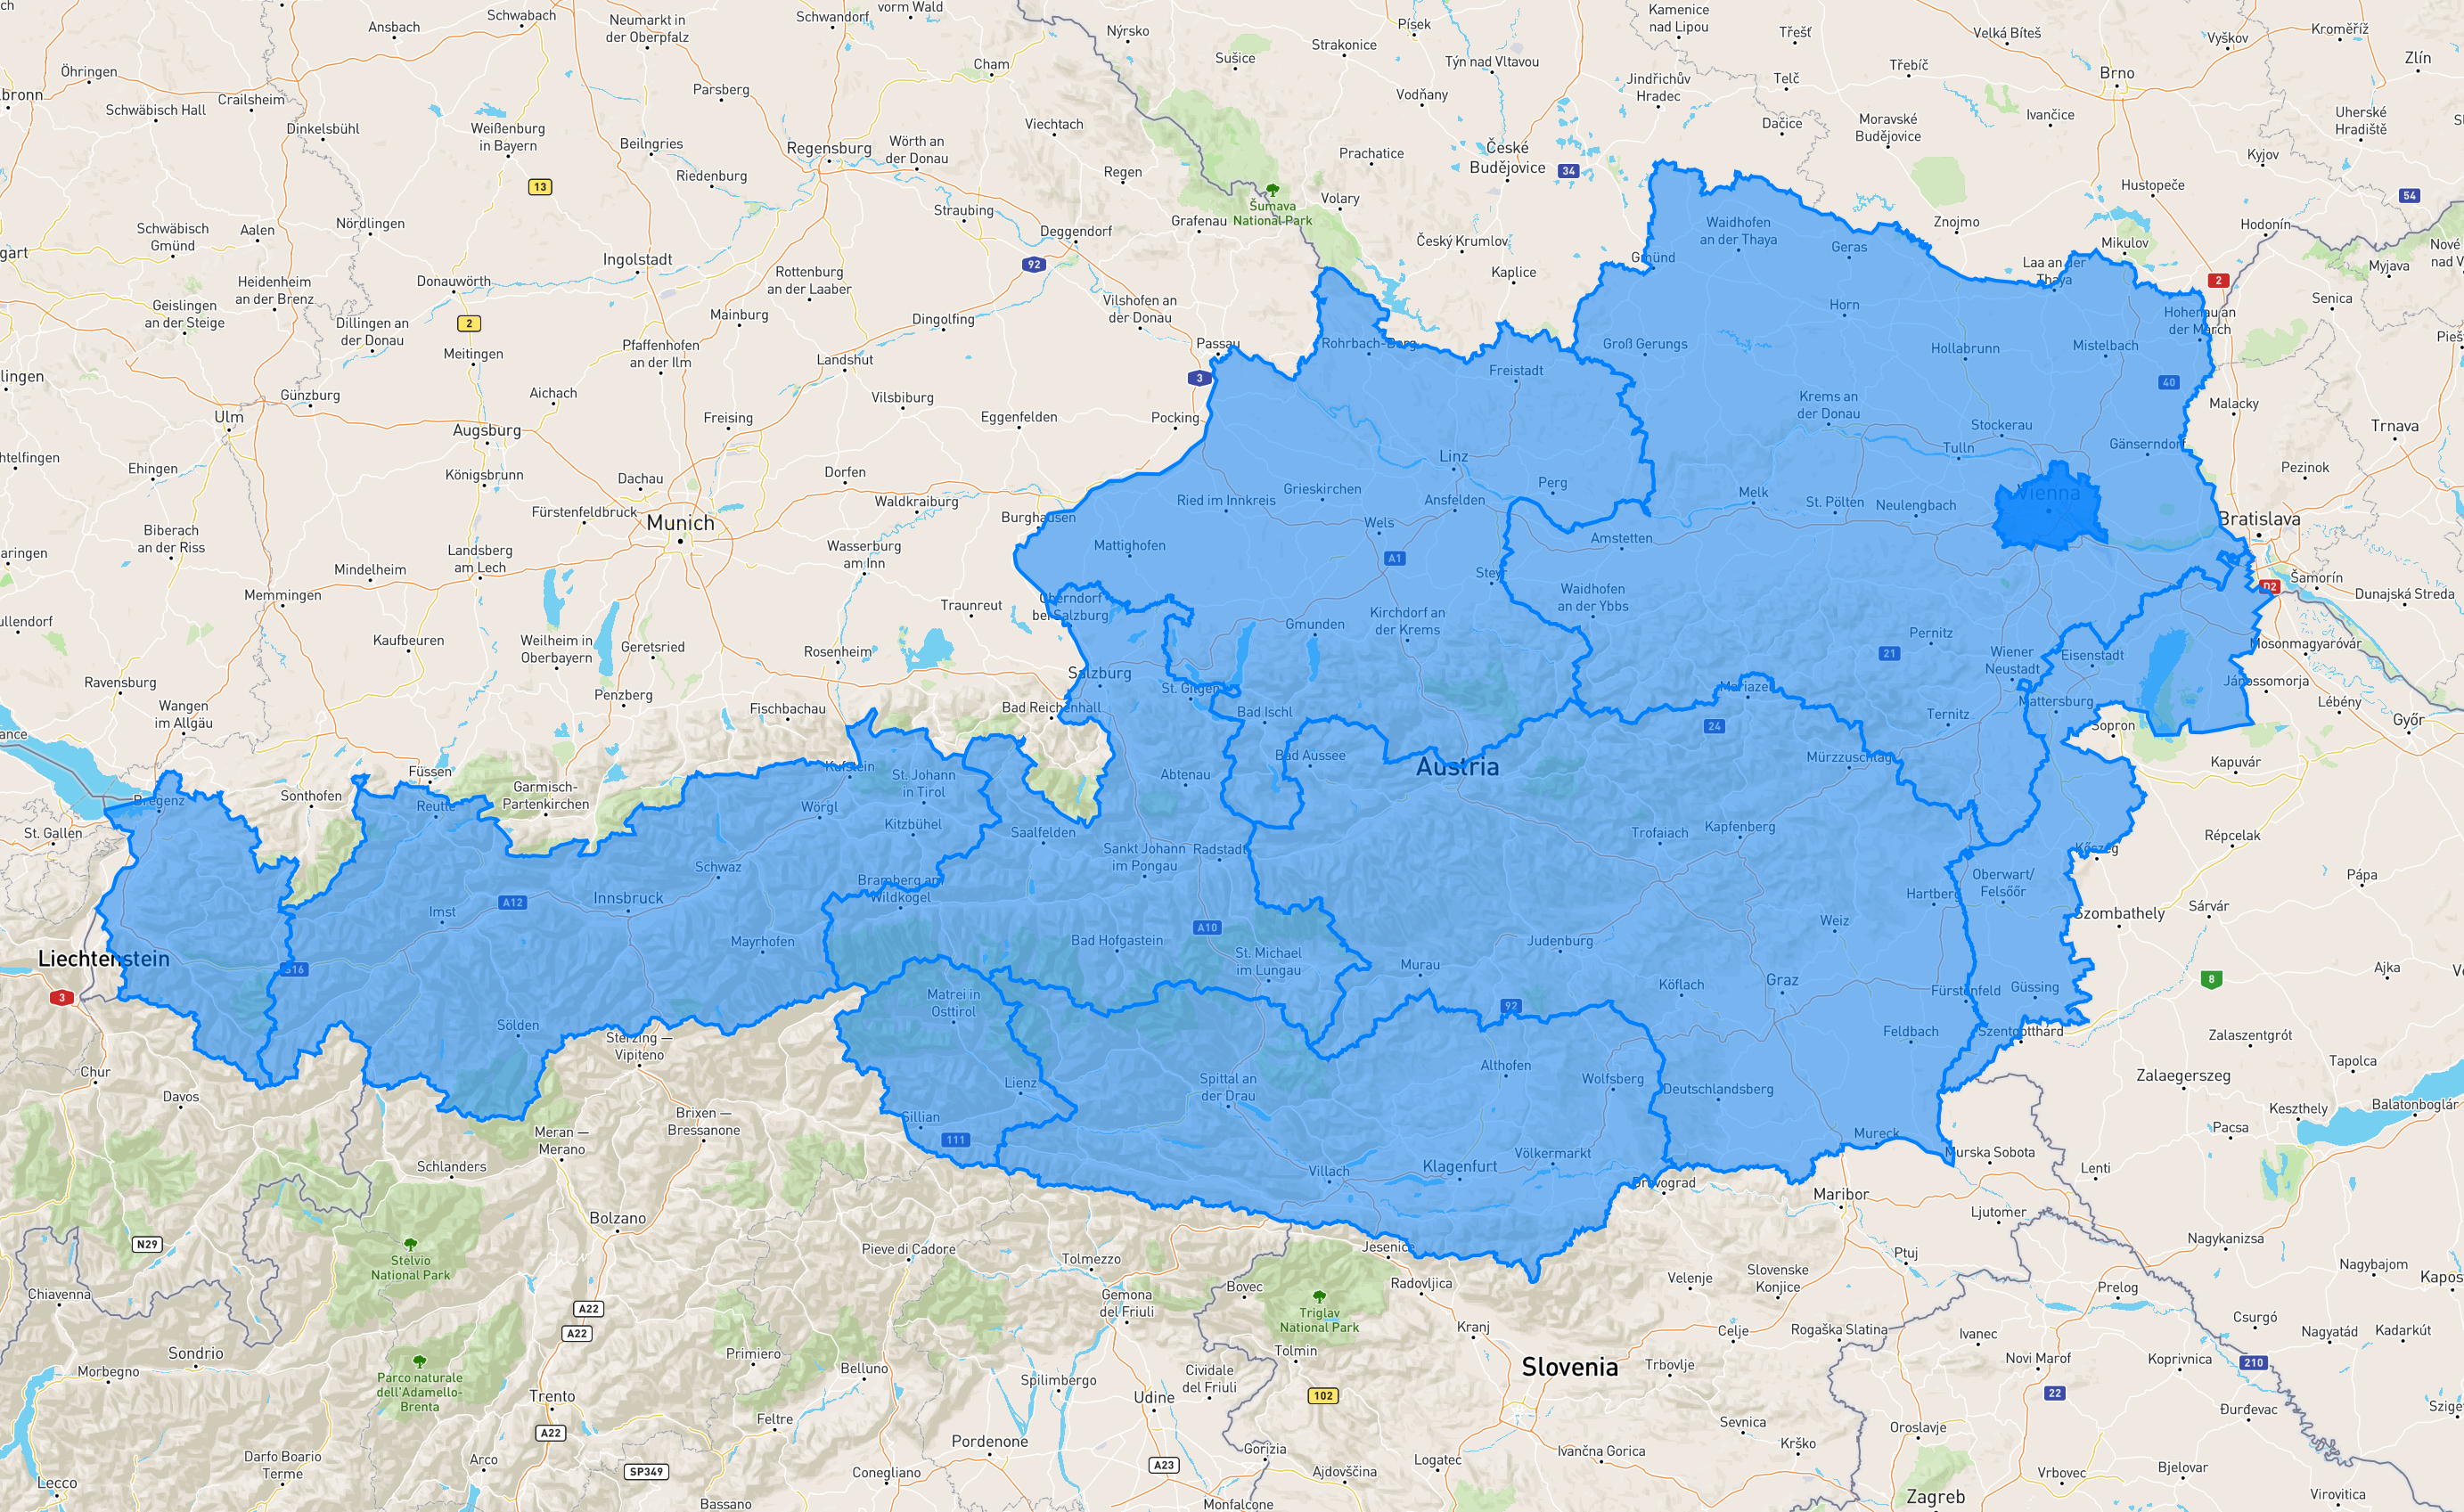
\includegraphics[scale=0.25]{pics/austria-mapbox}
    \caption{Österreich mit Bundesländern in Mapbox}
    \label{fig:austria-mapbox}
\end{figure}

\paragraph{Vorteile}
\begin{itemize}
    \item OpenSource (bis Version 2.0.0)~\cite{mapbox-open-source}
    \item Gutes Handling von großen Datensätzen
    \item Individualisierbar
    \item Gute Unterstützung von komplexen Strukturen
\end{itemize}

\paragraph{Nachteile}
\begin{itemize}
    \item Ausbaufähige Dokumentation
    \item Kein ausgereifter Angular Wrapper
\end{itemize}

\subsection{Leaflet}
Leaflet ist das laut eigenen Angaben die führende Open-Source JavaScript Library, wenn mobile und interaktive Karten gefordert sind.
Durch die sehr gute API Dokumentation können ganz leicht Geo-Daten auf Karten dargestellt und interaktive Elemente eingebaut werden.
Der Fokus liegt dabei auf den Grundfunktionalitäten, das beinhaltet auch eine Performance Optimierung für fast alle Geräte und Plattformen.
Dank einer leichten Anbindungsmöglichkeit für Plugins, gibt es etliche davon im Internet, die man einfach verwenden kann,
um die Funktionalitäten zu erweitern.
Leaflet wird auch von den ganz großen verwendet: GitHub, Pinterest, Facebook, European Commission, The Washington Post und noch viele mehr.
~\cite{leaflet-doc}

\begin{figure}[hbt!]
    \centering
    
\includegraphics[scale=0.4]{pics/austria-leaflet}
    \caption{Österreich mit Bundesländern in Leaflet}
    \label{fig:austria-leaflet}
\end{figure}

\paragraph{Vorteile}
\begin{itemize}
    \item Open-Source (keine Restriktion oder Terms of Service)
    \item Hervorragende Dokumentation
    \item Leichtgewichtig (39KB)
    \item Plugin Support
    \item Angular Wrapper
    \item Bereits von triply in Verwendung
\end{itemize}

\paragraph{Nachteile}
\begin{itemize}
    \item Offizielle Dokumentation beinhaltet nur grundlegende Beispiele
    \item Möglicherweise verwenden von GIS Programmen (zum Beispiel QGIS) notwendig, um Informationen aufzubereiten
\end{itemize}

\subsection{Google Maps}
Google Maps ist der Kartendienst von Google und der Kartenprovider mit den meisten Daten, welche zur Verfügung stehen.
OpenStreetMap ist vergleichsweise auf dem Globus nicht deckend, das liegt, jeder kann aber Daten oder Orte beisteuern.
Google Maps hingegen, hat Daten bis in jede noch so kleine Straße, das ermöglicht eine sehr gute Informationslage.
In Kombination mit Places API und der Maps images API kann niemand mit Google mithalten.
Das liegt auch daran, dass Google mehr als Maps betreut und deshalb viel mehr Möglichkeiten als zum Beispiel OpenStreetMap hat.
Der wohl größte Nachteil liegt an der kostenpflichtigen Nutzung ab einer gewissen Nutzerzahl.
Ab 1000 Anfragen pro Monat ist Google Maps nicht mehr gratis und damit frei zu nutzen~\cite{google-maps-vs-osm}.

\begin{figure}[hbt!]
    \centering
    \includegraphics[scale=0.2]{pics/austria-googlemaps}
    \caption{Österreich mit Bundesländern in Google Maps}
    \label{fig:austria-googlemaps}
\end{figure}

\paragraph{Vorteile}
\begin{itemize}
    \item Google Ökosystem
    \item hohe Abdeckung des Globus
    \item Angular Wrapper
\end{itemize}

\paragraph{Nachteile}
\begin{itemize}
    \item Kann kostenpflichtig werden
    \item Terms of Use und Restriktionen
    \item Google Logo immer sichtbar
    \item Farbschema kann kaum verändert werden.
\end{itemize}

\cleardoublepage

\subsection{Performance im Vergleich}
Um eine Wahl auf ein bestimmtes Framework treffen zu können, wurden mithilfe der Chrome-Developer-Tools die Ladezeiten
unter bestimmten Voraussetzungen der einzelnen Frameworks getestet.
In diesen Tools gibt es die Möglichkeit zwischen einem schnellem (fast), einem mittel-schnellem (mid-tier) und einem
langsamen (low-end) Gerät zu wählen.
Dadurch änderten sich die Ladezeiten teils sehr drastisch.
Folgende Ergebnisse wurden bei dem Versuch erhalten:

\begin{table}[hbt!]
    \centering
    \begin{tabular}{llll}
        & \textbf{Leaflet} & \textbf{Mapbox} & \textbf{Google Maps} \\
        \textbf{low-end device}  & 132s             & 138s            & 192s                 \\
        \textbf{mid-tier device} & 39,5s            & 41,69s          & 56,12s               \\
        \textbf{fast device}     & 1,2s             & 3,9s            & 3,23s
    \end{tabular}\label{tab:map-framework-table}
\end{table}

Aufgrund der oben genannten Vor- und Nachteilen, sowie persönlichen Erfahrungen der Entwickler und nach Absprache mit der
Betreuerfirma ist die Wahl schlussendlich auf Leaflet in Kombination mit einer Mapbox Tile-layer gefallen.
Tile-layers bestimmen die Darstellung der Karte an sich und werden von externen Servern direkt für den aktuell zu sehenden Bereich angefordert.

\cleardoublepage

\section{Static Site Generators}
\setauthor{Sebastian Scholl}
Um die Website zu generieren wurden verschiedene Static Site Generators analysiert.
Dabei wurde darauf geachtet, ob diese sich eignen, aufgrund von Geodaten eine Seite zusammenzubauen.

\subsection{Next.js}
Next.js ist eines der beliebtesten Frameworks, um statische Websites zu generieren.
Die Templates für diese Seiten werden jedoch in React geschrieben.
Vorteile von Next.js sind die einfache Installation und Flexibilität des Frameworks~\cite{nextjs}.

\subsection{Jekyll}
Jekyll ist ein Static Site Generator, der in Ruby geschrieben ist~\cite{jekyll-ruby}.
Im Gegensatz zu Next.js nutzt Jekyll kein JavaScript Framework, um die Templates zu erstellen, sondern setzt
auf \textit{Liquid}~\cite{jekyll-liquid}.
Es besteht zwar die Möglichkeit, es mit Angular zu verknüpfen.
Da aber Liquid und Angular beide mit doppelten geschwungenen Klammern arbeiten, um auf Variablen zuzugreifen, muss
dies in Angular geändert werden.
Das ist zwar grundsätzlich möglich, kann aber eine Sicherheitslücke darstellen und es wird davon abgeraten~\cite{angular-interpolation}.

Weiters wird Jekyll hauptsächlich für Blogs und Seite, die nur Text enthalten, verwendet.
Dementsprechend wird wenig Funktionalität für Seiten mit anderem Inhalt bereitgestellt.

\subsection{Scully}
Scully ist ein Static Site Generator, der auf Angular aufbaut.
Dabei liegt der Fokus jedoch auf serverseitigem Rendern und es werden keine weiteren Tools bereitgestellt, um auf
den Aufbau der Seite Einfluss zu nehmen.
Somit kann zwar die Zeit, die eine Seite braucht, um im Browser dargestellt zu werden, verringert werden, für das
dynamische Generieren der Seite eignet sich Scully aber nicht.

% TODO: evtl. kleine Community

\section{Deployment Pipeline}
\setauthor{Sebastian Scholl}
Nach dem Download des generierten Projekts sollte die Möglichkeit bestehen,
kleine Änderungen daran vorzunehmen und es dann schnell und einfach auf einen
Server zu deployen.
Der Server ist dabei entweder eine Linux Virtual Machine oder eine \textit{Firebase Hosting} Instanz.

Dazu gab es mehrere Ansätze: Ist das Projekt ein Git-Repository, kann eine
Automatisierungssoftware, wie Jenkins oder GitHub Actions verwendet werden,
die bei jedem \textit{Push}-Event das Projekt buildet und auf den Server
deployed.
 Die zweite Möglichkeit ist ein Node.js Skript, das im Projekt enthalten ist und von der Kommandozeile
 aus ausgeführt wird.

\subsection{SSH}
Secure Shell (SSH) ist ein Protokoll, das genutzt wird, um eine sichere Verbindung zwischen einem
Client und einem Server aufzubauen.
 Authentifizierung, Befehle, Output und Dateiübertragung sind dabei verschlüsselt.
 Das Protokoll wird typischerweise benutzt, um Befehle auf einem anderen Computer auszuführen und Dateien sicher
 zu übertragen.
 Dabei eignet es sich gut, um solche Prozesse zu automatisieren und wird daher oft in Continuous Integration und
Continuous Deployment Pipelines verwendet.

Das Protokoll arbeitet mit dem Client-Server-Modell.
 Das heißt, dass die Verbindung von einem SSH Client zu einem SSH Server aufgebaut wird.
 Mit einem Public Key wird die Identität des Servers sichergestellt.
 Nach dem Verbindungsaufbau werden die übertragenen Daten symmetrisch verschlüsselt und mithilfe von
 Hashing-Algorithmen wird die Integrität dieser Daten sichergestellt~\cite{ssh}.

Dateiübertragung über SSH wird mithilfe des SSH File Transfer Protocols (SFTP) realisiert.

\subsubsection{SSH Keys}
Benutzer und Benutzerinnen können zwischen verschiedenen Formen der Authentifizierung wählen.
Die beliebtesten Methoden sind Passwort-basierte Authentifizierung und Public Key Authentifizierung.
Letztere wird vor allem bei automatisierten Prozessen eingesetzt.
Dabei haben der Benutzer oder die Benutzerin ein kryptografisches Schlüsselpaar.
Dieses besteht aus Public Key und Private Key.
Der Public Key wird am Server hinterlegt und jeder mit einer Kopie des dazu passenden Private Keys kann
auf diesen Server zugreifen~\cite{ssh-keys}.

\subsection{Firebase Hosting}
Firebase ist ein Backend-as-a-Service (BaaS), das von Google angeboten wird.
 Es besteht aus verschiedenen Produkten, die Softwareentwicklern und Softwareentwicklerinnen das Entwickeln
von Backends ermöglicht, ohne sich um Server kümmern zu müssen.
 Beispiele für Produkte sind Firebase Authentication, das eine einfache Authentifizierung von Usern ermöglicht,
Realtime Database, eine NoSQL Datenbank oder Firebase Hosting, das das Hosten von Webanwendungen,
statischen Websites oder Microservices übernimmt~\cite{firebase}.

Firebase Hosting ist für eine Verwendung von bis zu 10 GB Speicherplatz gratis~\cite{firebase-pricing}
und stellt mit der Firebase CLI einen einfachen und schnellen Weg zur Verfügung, die gewünschten
Dateien hochzuladen.
Es eignet sich somit für das Hosten der generierten Websites. Weitere Vorteile sind, dass für jedes Firebase
Hosting Projekt eine eigene Domain zur Verfügung gestellt
wird und dass die Website auf das globale Content Delivery Network (CDN) verteilt wird, um
die Ladegeschwindigkeiten zu erhöhen~\cite{firebase-hosting}.

\subsection{Jenkins}
Jenkins ist ein Open-Source Automatisierungsserver.
Das Projekt wird in Java entwickelt und kann mithilfe von Plugins an spezifische Anforderungen
angepasst werden~\cite{jenkins-github}.

Der Server wird vor allem zur Automatisierung von Aufgaben, wie das Builden,
Testen und Deployen von Softwareprojekten genutzt.
Jenkins muss selbst gehosted werden.
 Dazu wird ein offizielles Docker Image im Docker Hub bereitgestellt~\cite{jenkins-dockerhub}.

Die Konfiguration einer Pipeline wird in einem \textit{Jenkinsfile} vorgenommen,
das sich im Git-Repository des Projekts befindet.
 Darin werden mehrere sogenannte Stages definiert, die dann nacheinander ausgeführt werden.
 Jede Stage ist wiederrum in mehrere Steps gegliedert, die verschiedene Aufgaben übernehmen und auch in der
definierten Reihenfolge ausgeführt werden.

Eine Pipeline mit den Stages \textit{Build}, \textit{Test} und \textit{Deploy} würde
zum Beispiel folgendermaßen aussehen: ~\cite{jenkins-jenkinsfile}

\begin{lstlisting}[numbers=left]
pipeline {
    agent any

    stages {
        stage('Build') {
            steps {
                echo 'Building..'
            }
        }
        stage('Test') {
            steps {
                echo 'Testing..'
            }
        }
        stage('Deploy') {
            steps {
                echo 'Deploying....'
            }
        }
    }
}
\end{lstlisting}

\subsection{GitHub Actions}
GitHub Actions ist eine Automatisierungssoftware, die von GitHub zur Verfügung
gestellt wird.
Im Gegensatz zu Jenkins werden die Server dabei von GitHub gehostet.
Die Konfiguration von sogenannten Workflows wird in \textit{YAML}-Dateien im
\textit{.github/workflows} Directory eines Repositories vorgenommen.

GitHub Actions sind tief in das GitHub Ökosystem integriert und bieten viele Möglichkeiten,
auf verschiedene Teile davon zuzugreifen.
 Damit können Workflows erstellt werden, die nicht nur die Software builden, testen und deployen, sondern auch
 zum Beispiel die Labels von Issues verändern.

Ein Workflow enthält einen oder mehrere Jobs, die sequentiell oder parallel ausgeführt werden
können.
 Jeder Job läuft auf einer eigenen Virtuellen Maschine, auch Runner genannt und ist in
verschiedene Actions unterteilt, die wiederrum mehrere Steps enthalten.
 Dabei läuft
auf den Runnern entweder Windows, Linux oder macOS als Betriebssystem.

Ein Workflow, der bei jedem Push oder Pull Request auf den \textit{main} Branch die Steps
\textit{Build}, \textit{Test} und \textit{Deploy} ausführt könnte beispielsweise folgendermaßen
aussehen: ~\cite{github-actions}

\begin{lstlisting}[numbers=left]
name: Build & Deploy

on:
  push:
    branches: [ main ]
  pull_request:
    branches: [ main ]

jobs:
  build-deploy:
    runs-on: ubuntu-latest
    steps:
    - uses: actions/checkout@v2
    - name: Build
      run: echo Building
    - name: Test
      run: echo Testing
    - name: Deploy
      run: echo Deploy
\end{lstlisting}

\subsubsection{Secrets}
Secrets sind verschlüsselte Umgebungsvariablen, die für eine GitHub Organisation oder ein
Repository erstellt werden.
Darin können sensible Informationen, wie z.B. Passwörter oder Private Keys gespeichert werden.
Diese Secrets sind dann in GitHub Actions Workflows verfügbar.
GitHub stellt sicher, dass Secrets verschlüsselt werden, bevor sie die GitHub Server erreichen
und verschlüsselt bleiben, bis sie in einem Workflow verwendet werden~\cite{github-secrets}.

\begin{figure}[hbt!]
    \centering
    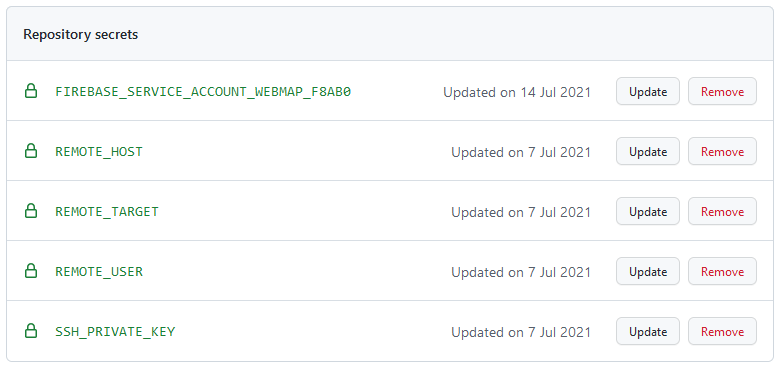
\includegraphics[scale=0.5]{pics/secrets.png}
    \caption{Repository secrets}
\end{figure}

In folgendem Step eines Workflows werden diese Secrets dann referenziert:

\begin{lstlisting}[numbers=left]
- name: Deploy to Server
  uses: easingthemes/ssh-deploy@v2
  env:
    SSH_PRIVATE_KEY: ${{ secrets.SSH_PRIVATE_KEY }}
    SOURCE: static/
    REMOTE_HOST: ${{ secrets.REMOTE_HOST }}
    REMOTE_USER: ${{ secrets.REMOTE_USER }}
    TARGET: ${{ secrets.REMOTE_TARGET }}
\end{lstlisting}

\subsection{Node.js Skripts}
Node.js~\ref{Node.js} Skripts haben den Vorteil gegenüber dem Ansatz mit einer Automatisierungssoftware,
dass dafür kein GitHub Repository erstellt werden muss und nur die Kommandozeile benötigt wird.
Da Node.js plattformunabhängig ist, können diese Skripts in sowohl auf Windows als auch auf
Linux und macOS ausgeführt werden.

 \section{JSON}
 JavaScript Object Notation (JSON) ist ein Format zum Datenaustausch.
 Es wurde entworfen, um für Menschen einfach zu lesen und zu schreiben zu sein.
 Außerdem ist es auch für Maschinen einfach zu parsen oder zu generieren.
 Das Format ist unabhängig von Programmiersprachen.

 JSON baut auf zwei Strukturen auf:

 \begin{itemize}
     \item Object: Eine Sammlung an Key/Value Paaren.
     In den meisten Programmiersprachen wird das als Object, Record, Struct
     oder Dictionary umgesetzt.
     \item Array: Eine geordnete Sammlung an Werten.
     Diese Struktur wird als Array, Vector, List oder Sequence umgesetzt.
 \end{itemize}

 Ein Object ist ein ungeordnetes Set an Key/Value Paaren.
 Es beginnt mit \textit{{} und endet mit \textit{}}.
 Die darin enthaltenen Werte haben das Format \textit{key: value} und werden mit Beistrichen voneinander getrennt.
 Der Key ist immer ein String und muss deshalb in Anführungszeichen stehen.

 Ein Array ist eine geordnete Sammlung an Werten.
 Es startet mit \textit{[} und wird mit \textit{]} beendet.
 Die darin enthaltenen Werte werden wiederrum mit Beistrichen getrennt.

 Werte können ein String sein, der in Anführungszeichen steht, eine Zahl, \textit{true}, \textit{false}, \textit{null}
 oder wieder ein Object oder Array~\cite{json}.

 Ein valides JSON-Object könnte also folgendermaßen aussehen:

 \label{json-example}
 \begin{lstlisting}[numbers=left]
{
  "string": "Hello World",
  "number": 69,
  "boolean": false,
  "null": null,
  "array": [
    419,
    420,
    "421",
    null
  ]
}
 \end{lstlisting}

 \subsection{JSON-Schema}
Ein JSON Schema wird dazu verwendet, JSON Strukturen zu beschreiben und zu validieren.
Damit kann beispielsweise eine Dokumentation für eine Schnittstelle, die über JSON kommuniziert, definiert werden.
Diese Dokumentation ist dabei sowohl für Menschen, als auch für Maschinen einfach lesbar.
Ein weiterer Einsatzbereich von JSON-Schemata ist das Validieren von Daten bei automatisierten Tests~\cite{json-schema}.

 Ein JSON-Schema ist selbst wiederrum nur ein JSON-Object.
 Dieses besitzt meistens einen \textit{title} und eine \textit{description}, die das definierte JSON beschreiben,
 aber keine Auswirkung auf die Struktur haben.
 Das \textit{type} Keyword definiert den Typ einer Property.
 Dieser kann entweder "null", "boolean", "object", "array", "number", oder "string" sein.

 Ist der Typ "object", muss dieses Object weiter beschrieben werden.
 Dazu wird das \textit{properties} Keyword verwendet.
 Der Wert davon ist ein Object mit den Properties des zu beschreibenden Object als Keys.
 Die Werte dieser Keys sind wiederrum Objects, die die jeweilige Property beschreiben.
 Dazu wird wieder das \textit{type} Keyword verwendet.
 Mit dem \textit{description} Keyword kann man auch dieser Property wieder eine Beschreibung geben.

 Eine Property vom Typ "array" beschreibt mit dem \textit{items} Keyword den Typ der Werte, die das Array enthält.

 Für die meisten Typen gibt es noch zusätzliche Keywords, mit denen die Werte noch genauer beschrieben werden können.
 Dazu zählen beispielsweise \textit{required} für Werte vom Typ "object", das ein Array der Namen der erforderlichen
 Properties enthält oder \textit{maximum} und \textit{minimum} für Werte vom Typ "number" bzw. "integer".

 Ein JSON-Schema für das JSON-Object aus dem vorherigen Kapitel~\ref{json-example} könnte beispielsweise
 folgendermaßen aussehen:

 \begin{lstlisting}[numbers=left]
    {
      "title": "Example JSON Object",
      "description": "A JSON Object to demonstrate JSON Syntax",
      "type": "object",
      "properties": {
        "string": {
          "description": "Some string",
          "type": "string"
        },
        "number": {
          "description": "Some number",
          "type": "integer",
          "maximum": 100
        },
        "boolean": {
          "description": "Some boolean",
          "type": "boolean"
        },
        "null": {
          "description": "Null",
          "type": "null"
        },
        "array": {
          "description": "Some array",
          "type": "array",
          "items": {
            "oneOf": [
              {
                "type": "number"
              },
              {
                "type": "string"
              },
              {
                "type": "null"
              }
            ]
          }
        }
      },
      "required": [ "string", "number", "array" ]
    }
 \end{lstlisting}

\section{Backend}
\setauthor{Sebastian Scholl}
Das Backend von webmap erfüllt zwei Aufgaben:

\begin{itemize}
    \item Das Hosten des Generators
    \item Eine REST-API für das Generieren eines Angular-Projekts aufgrund der im Generator erstellten Konfiguration
\end{itemize}

Für das Hosting wurde nginx verwendet und die REST-API wurde in TypeScript implementiert.

\subsection{TypeScript}
Um webmap leicht warten zu können, wurde auch das Backend in TypeScript~\ref{TypeScript} geschrieben.
 Damit wird nur eine Programmiersprache für das gesamte Projekt verwendet.
 Ausgeführt wird das Backend in der Laufzeitumgebung Node.js.
 Diese wurde entwickelt, um skalierbare Netzwerkanwendungen zu erstellen und eignet sich daher für
 die REST-API~\cite{about-node-js}.

\subsubsection{express.js}
Die API wurde mit dem Node-Package \textit{express.js} entwickelt.
 Express ist ein schnelles und minimalistisches Web Framework.
 Die Kernfunktion liegt darin, schnelle und robuste APIs zu entwickeln~\cite{expressjs}.

\subsubsection{node-tar}
Zum Komprimieren des generierten Projekts wird das Node-Package \textit{node-tar} verwendet.
 Das Package ahmt dabei den UNIX-Befehl \textit{tar} nach~\cite{node-tar}.

Ein \textit{tar}-File oder \textit{tarball} ist ein Archiv von Filesystem-Einträgen wie Dateien, Directories oder
Symbolic Links.
 Diese können dann noch komprimiert werden, um ein \textit{.tar.gz}-File zu erhalten.
 Tar wird hauptsächlich zur Distribution oder für Backups von mehreren Dateien verwendet~\cite{tar-manpage}.

 \subsubsection{ESLint}
 ESLint ist ein Open-Source Linting Tool für JavaScript und TypeScript.
 Es wird verwendet, um geschriebenen Code zu analysieren, um Muster zu finden, von denen man weiß, dass sie
 problematisch und anfällig für Bugs sind.
 Weiters kann man damit einen bestimmten Code Style definieren, um den Code konsistent und lesbar zu machen.
 Alle diese Aspekte werden als sogenannte Rules definiert.
 Die Library stellt eine Menge an vorgefertigten Rules zur Verfügung, es können aber auch sehr einfach eigene
 Rules erstellt werden~\cite{eslint}.

\section{nginx}
\setauthor{Sebastian Scholl}
nginx ist ein Open-Source HTTP Server, Reverse Proxy Server, Mail Proxy Server und generischer TCP/UDP Proxy Server.
Konfigurationen werden im \textit{/etc/nginx/nginx.conf} File durchgeführt.
 Standardmäßig stellt der Webserver alle Dateien im \textit{/usr/share/nginx/html} Directory Clients zur
 Verfügung~\cite{nginx}.
 Auch für nginx steht ein offizielles Docker Image am Docker Hub zur Verfügung~\cite{nginx-dockerhub}.

\subsubsection{Reverse Proxy}
Ein Reverse Proxy Server wie nginx befindet sich typischerweise hinter einer Firewall in einem
privaten Netzwerk und verteilt Requests von Clients auf die entsprechenden Backend Server.
Damit erhält man eine weitere Abstraktionsschicht, um den Verkehr zwischen Clients und Servern zu
verwalten und zu überwachen~\cite{nginx-proxy-server}.

nginx kann mit folgendem \textit{nginx.conf} File als Proxy Server konfiguriert werden, der Requests zu \textit{/api}
an einen anderen Server weiterleitet.
Bei allen anderen Requests wird eine Datei aus dem \textit{/data} Directory als Response gesendet.

\begin{lstlisting}[numbers=left]
events {}

http {
  include mime.types;

  server {
    location /api {
      proxy_pass http://localhost:4000/;
    }

    location / {
      root /data;
    }
  }
}
\end{lstlisting}

\section{Containerization}
\setauthor{Sebastian Scholl}
\subsection{Docker}
 Docker ist eine Softwareplattform, die Benutzern und Benutzerinnen erlaubt, Applikationen schnell zu
 Builden, Testen und Deployen.
 Dabei wird die Software in standardisierte Pakete, die Container genannt werden, verpackt~\cite{docker-aws}.

\subsubsection{Container}
 Container sind abgeschlossene Systeme, die Software sowie die gesamte Infrastruktur, die diese Software
 benötigt, um zu laufen, enthält.
 Dazu gehören Libraries, sowie eine Laufzeitumgebung.
 Die Idee von Containern erinnert an Virtuelle Maschinen.
 Bei Containern wird jedoch das Betriebssystem virtualisiert, im Gegensatz zu Virtuellen Maschinen,
 bei denen die Hardware virtualisiert wird.
 Deshalb benötigt jede VM eine eigene Kopie eines Betriebssystemes, was mehrere GB an Speicherplatz beansprucht.
 Container haben hingegen typischerweise eine Größe von weniger als 100 MB~\cite{docker-container}.

 \begin{figure}[hbt!]
     \centering
     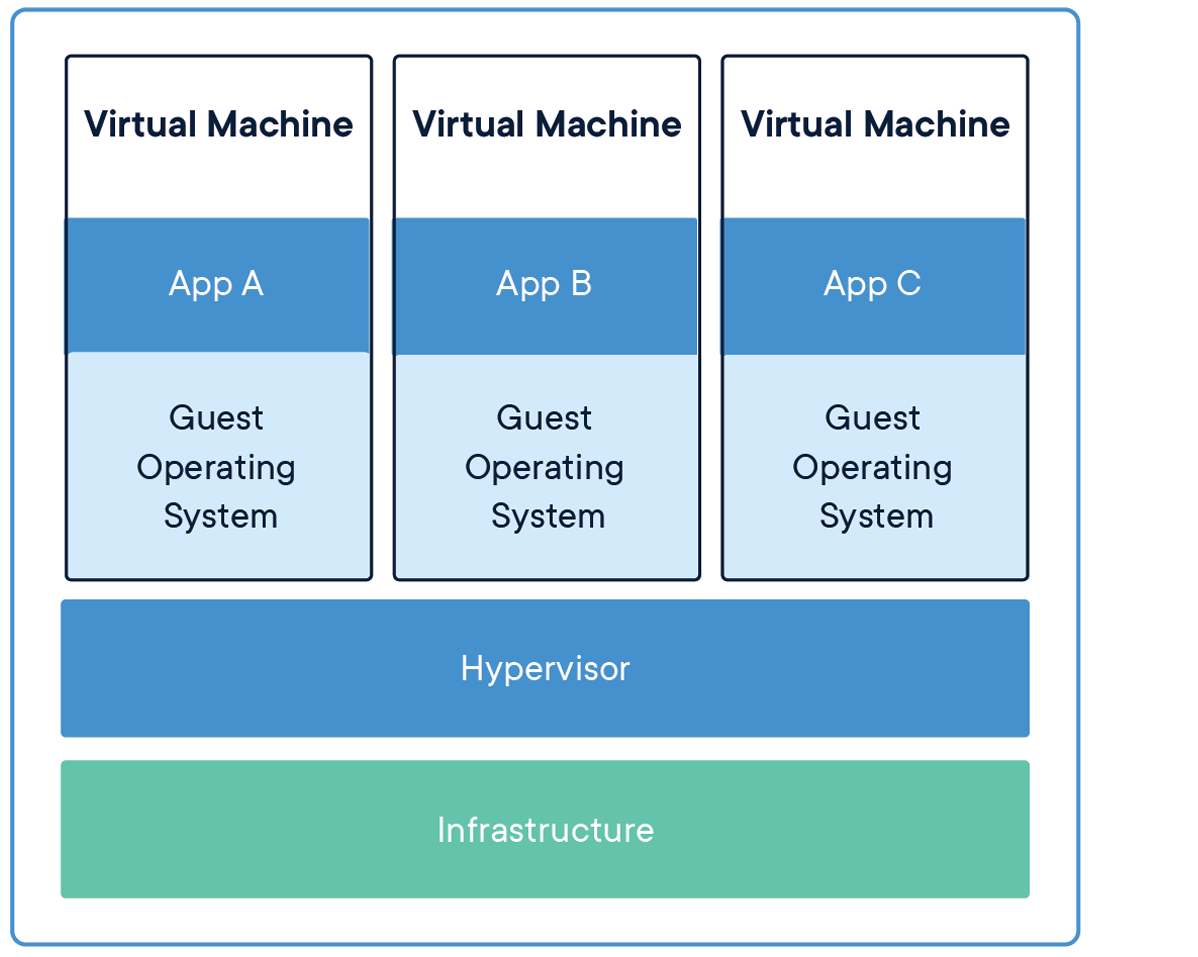
\includegraphics[scale=0.2]{pics/docker-vm.png}
     \caption{Virtualisierung mit Virtuellen Maschinen}
     % Source: https://www.docker.com/resources/what-container/, 25.03.
 \end{figure}

 \begin{figure}[hbt!]
     \centering
     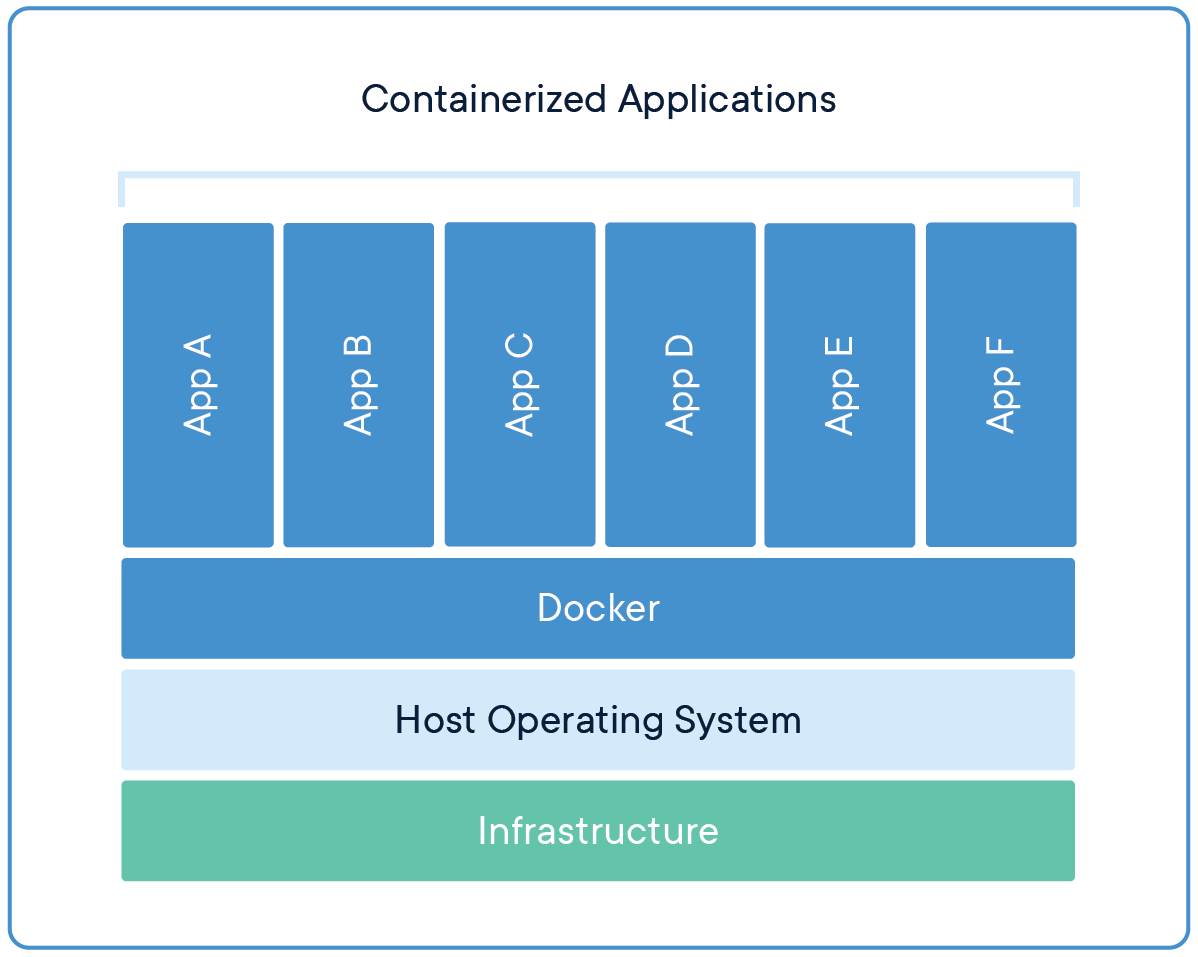
\includegraphics[scale=0.2]{pics/docker-containerized.png}
     \caption{Virtualisierung mit Containern}
     % Source: https://www.docker.com/resources/what-container/, 25.03.
 \end{figure}

\subsubsection{Image}
 Container werden aus sogenannten Images erstellt.
 Diese Images erhalten alles, was ein Container benötigt, um zu laufen.
 Dazu gehören das Filesystem mit allen Dependencies und Konfigurationen, Umgebungsvariablen
 und einen Befehl, um die Software im Container zu starten.
 Beim Start des Containers wird der Inhalt des Images kopiert und darin der Befehl ausgeführt, der die Software
 startet.
 Dafür wird der Docker CLI Befehl \textit{docker run [image name]} verwendet~\cite{docker-image}.

 Images können entweder von einem Registry heruntergeladen oder selbst in einem sogenannten \textit{Dockerfile}
 definiert werden.
 Jedes \textit{Dockerfile} startet mit einem Base Image, auf dem aufgebaut wird.
 Danach können zum Beispiel Files in das Image kopiert werden, aus denen dann eine Applikation gebuildet wird.
 Zum Schluss benötigt ein \textit{Dockerfile} noch einen Befehl, der beim Start eines Containers ausgeführt wird.

 Folgendes Dockerfile verwendet das Base Image \textit{ubuntu}.
 Das gesamte Directory, in dem sich das \textit{Dockerfile} befindet, wird daraufhin in das \textit{/app} Directory
 des Images kopiert.
 Darin wird der \textit{make} Befehl ausgeführt, um die Applikation zu builden.
 Als Befehl, der beim Start ausgeführt wird, wird \textit{python /app/app.py} definiert~\cite{dockerfile}.

 \begin{lstlisting}[numbers=left]
  FROM ubuntu:18.04
  COPY . /app
  RUN make /app
  CMD python /app/app.py
 \end{lstlisting}

 \subsubsection{Persistierung}
 Docker bietet zwei Wege an, um Daten, die in Containern generiert werden, zu persistieren.
 Bind Mounts synchronisieren ein Directory im lokalen Filesystem mit einem Directory im Filesystem des Containers.
 Diese Bind Mounts werden jedoch öfter dazu verwendet, um Daten von außerhalb in den Container zu kopieren.

 Um Daten, die im Container generiert werden, zu persistieren werden meistens Volumes verwendet.
 Volumes enthalten ein Directory des Containers und werden vollständig von Docker verwaltet.
 Wird der Container gestoppt oder gelöscht, bleiben die Daten im Volume erhalten.

 Volumes werden beim Erstellen des Containers konfiguriert.
 Die Docker CLI stellt dafür die \textit{-v} bzw. \textit{--volume} Flag zur Verfügung~\cite{docker-volumes}.

 \subsubsection{Microservices}
 Microservices beschreibt einen Ansatz in der Softwareentwicklung, bei dem die Software in kleine, unabhängige
 Services aufgeteilt ist, die über definierte APIs miteinander kommunizieren.
 Diese Architektur machen Applikationen leichter skalierbar.
 Diese Services werden oft als Docker Container realisiert.

 Das Gegenteil der Microservice Architektur ist ein Monolith.
 Dabei ist die gesamte Applikation ein einzelner Service.
 Dieser enthält alle Komponenten, die eng miteinander verbunden sind.
 Bei erhöhter Auslastung muss dann die gesamte Applikation skaliert werden.
 Jede zusätzliche Komponente erhöht außerdem die Komplexität des gesamten Services.
 Das macht es schwieriger, mit neuen Technologien zu experimentieren und neue Ideen einzubauen.
 Durch die Abhängigkeit der Komponenten voneinander kann ein einzelner Fehler in einem Teil des Services eine
 große Auswirkung auf die gesamte Applikation haben.

 Microservices sollen diese Probleme lösen.
 Die Komponenten funktionieren unabhängig von einander und so muss bei der erhöhten Auslastung eines Services nur
 dieser skaliert werden.
 Da die Services über eine definierte API miteinander kommunizieren kann die Technologie in den Services einfach
 ausgetauscht werden.
 Weiters beschränken sich die Ausmaße von Fehlern nur auf den Service, in dem sie auftreten.

 Mit der steigenden Verbreitung von Cloud Computing werden Microservices immer beliebter, da die Skalierung
 von Services dabei automatisiert werden kann~\cite{microservices}.

 \begin{figure}[hbt!]
     \centering
     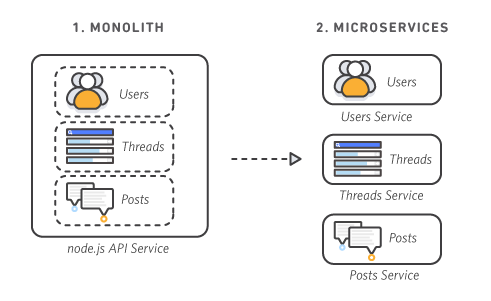
\includegraphics[scale=0.5]{pics/microservice.png}
     \caption{Monolith vs. Microservices}
     % Source: https://aws.amazon.com/microservices/, 25.03.
 \end{figure}

 \subsubsection{Docker Hub}
 Docker Images können in sogenannte Registries hochgeladen und so verteilt werden~\cite{docker-registry}.
 Das größte Registry ist der Docker Hub~\cite{docker-hub}.
 Darin werden auch offizielle Images für Softwarepakete, wie Ubuntu, nginx oder Node.js zur Verfügung gestellt.
 Diese Images werden immer auf dem neusten Stand gehalten, um die Sicherheit zu
 gewährleisten~\cite{docker-official-images}.

\subsection{Docker Compose}

 Docker Compose ist ein Tool zur Orchestrierung von Docker Containern.
 Es wird verwendet, um Applikationen mit mehreren Containern zu verwalten.
 In einem \textit{YAML} File werden die Services der Applikation definiert, die dann alle mit einem einzelnen
 Befehl gestartet werden können~\cite{docker-compose}.

 \subsubsection{Networking}
 Alle Services, die im gleichen File definiert werden, befinden sich automatisch im selben Docker Netzwerk.
 Das bedeutet, dass die miteinander kommunizieren können, aber nicht von außen auf sie zugegriffen werden kann.
 Jeder Service kann jedoch einzelne Ports definieren, die auch von außerhalb erreichbar sein sollen.
 Diese Abstraktionsschicht erhöht die Sicherheit, da zum Beispiel nur Services innerhalb eines Docker Netzwerks auf eine
 Datenbank zugreifen können, diese von Prozessen außerhalb nicht erreichbar ist.
 Docker Compose erleichtert das Routing innerhalb der Docker Netzwerke außerdem, indem der Hostname eines Services
 gleich seinem Namen ist~\cite{docker-network}.
